\documentclass[12pt,a4paper,oneside]{report}

% XeLaTeX document: Vietnamese academic report, A4 portrait.
\usepackage[a4paper,left=27mm,right=23mm,top=24mm,bottom=24mm,headheight=15pt]{geometry}
\usepackage{fontspec}
\IfFontExistsTF{Times New Roman}{\setmainfont{Times New Roman}}{\setmainfont{TeX Gyre Termes}}
\IfFontExistsTF{Arial}{\setsansfont{Arial}}{\setsansfont{TeX Gyre Heros}}
\usepackage{graphicx}
\usepackage{xcolor}
\usepackage{booktabs}
\usepackage{tabularx}
\usepackage{longtable}
\usepackage{array}
\usepackage{enumitem}
\usepackage{listings}
\usepackage{tikz}
\usetikzlibrary{arrows.meta}
\usepackage{fancyhdr}
\usepackage{titlesec}
\usepackage{hyperref}

\definecolor{navy}{HTML}{17324D}
\definecolor{teal}{HTML}{167D8D}
\definecolor{pale}{HTML}{EEF4F7}
\definecolor{codebg}{HTML}{F5F7F8}
\definecolor{codeframe}{HTML}{CBD5DC}
\hypersetup{colorlinks=true,linkcolor=navy,urlcolor=teal,citecolor=navy,pdftitle={Đặc tả phần mềm Billing-app},pdfsubject={Bài tập lớn môn Đặc tả phần mềm}}

\setlength{\parindent}{1.1em}
\setlength{\parskip}{4pt}
\setcounter{secnumdepth}{3}
\setcounter{tocdepth}{2}
\setlist{nosep,leftmargin=1.6em,topsep=2pt,partopsep=0pt}
\widowpenalty=10000
\clubpenalty=10000
\brokenpenalty=10000
\emergencystretch=2em
\setlength{\tabcolsep}{3pt}
\renewcommand{\arraystretch}{1.12}
\titleformat{\chapter}[display]{\bfseries\centering\color{navy}}{\large CHƯƠNG \thechapter}{4pt}{\Large}
\titlespacing*{\chapter}{0pt}{-10pt}{14pt}
\titleformat{\section}{\bfseries\large\color{navy}}{\thesection}{0.7em}{}
\titleformat{\subsection}{\bfseries\normalsize\color{teal}}{\thesubsection}{0.7em}{}

\pagestyle{fancy}
\fancyhf{}
\fancyhead[L]{\small\nouppercase{ĐẶC TẢ PHẦN MỀM — BILLING-APP}}
\fancyhead[R]{\small\nouppercase{Bài tập lớn}}
\fancyfoot[C]{\small\thepage}
\renewcommand{\headrulewidth}{0.35pt}
\renewcommand{\footrulewidth}{0pt}
\fancypagestyle{plain}{\fancyhf{}\fancyhead[L]{\small ĐẶC TẢ PHẦN MỀM — BILLING-APP}\fancyfoot[C]{\small\thepage}\renewcommand{\headrulewidth}{0.35pt}}

\lstdefinestyle{mermaid}{
  basicstyle=\ttfamily\footnotesize,
  backgroundcolor=\color{codebg},
  frame=single,
  rulecolor=\color{codeframe},
  numbers=left,
  numberstyle=\tiny\color{gray},
  numbersep=6pt,
  breaklines=true,
  breakatwhitespace=false,
  keepspaces=true,
  showstringspaces=false,
  columns=fullflexible,
  xleftmargin=1em,
  framexleftmargin=0.7em,
  aboveskip=6pt,
  belowskip=8pt
}
\lstdefinestyle{pseudo}{
  basicstyle=\ttfamily\small,
  backgroundcolor=\color{codebg},
  frame=single,
  rulecolor=\color{codeframe},
  breaklines=true,
  columns=fullflexible,
  keepspaces=true,
  showstringspaces=false,
  xleftmargin=0.5em,
  aboveskip=5pt,
  belowskip=7pt
}

\newcolumntype{Y}{>{\raggedright\arraybackslash}X}
\newcolumntype{D}[1]{>{\raggedright\arraybackslash}p{#1}}
\newcommand{\UC}[6]{%
\par\medskip\noindent\begin{tabularx}{\textwidth}{@{}>{\bfseries\color{navy}}p{3.0cm}Y@{}}\toprule
Mã UC & #1\\
Tác nhân & #2\\
Tiền điều kiện & #3\\
Luồng sự kiện chính & #4\\
Luồng rẽ nhánh / ngoại lệ & #5\\
Hậu điều kiện & #6\\
\bottomrule\end{tabularx}\par\smallskip
}
\newcommand{\ClassTableTitle}[1]{\par\medskip\noindent\textbf{#1}\par\smallskip}
\newcommand{\Source}[1]{\textit{Căn cứ mã nguồn: }\path{#1}.}
\newcommand{\Card}[1]{\textcolor{teal}{\textbf{#1}}}
\renewcommand{\contentsname}{Mục lục}
\renewcommand{\listfigurename}{Danh mục hình}
\renewcommand{\listtablename}{Danh mục bảng}
\renewcommand{\tablename}{Bảng}
\renewcommand{\figurename}{Hình}
\renewcommand{\bibname}{Tài liệu tham khảo}

\begin{document}

\begin{titlepage}
\thispagestyle{empty}
\begin{center}
\vspace*{12mm}
{\Large\bfseries BÀI TẬP LỚN}\par
\vspace{3mm}
{\large MÔN HỌC: ĐẶC TẢ PHẦN MỀM}\par
\vspace{21mm}
{\large HỆ THỐNG QUẢN LÝ BÁN HÀNG BILLING-APP}\par
\vspace{5mm}
{\Huge\bfseries\color{navy} ĐẶC TẢ YÊU CẦU VÀ THIẾT KẾ}\par
\vspace{3mm}
{\Large Mô hình miền, lớp chi tiết và cơ sở dữ liệu}\par
\vspace{18mm}

\begin{tikzpicture}
\draw[teal,line width=1.2pt] (0,0) -- (10,0);
\draw[navy,line width=0.35pt] (0,-0.18) -- (10,-0.18);
\end{tikzpicture}\par
\vspace{14mm}
\begin{tabular}{rl}
\textbf{Đối tượng khảo sát:} & Billing-app (React/Vite và Spring Boot)\\[4mm]
\textbf{Học phần:} & Đặc tả phần mềm\\[4mm]
\textbf{Phiên bản khảo sát:} & Mã nguồn hiện có tại ngày 24/09/2026\\
\end{tabular}
\vfill
{\large HÀ NỘI — 2026}\par
\end{center}
\end{titlepage}

\pagenumbering{roman}
\chapter*{TÓM TẮT}
\addcontentsline{toc}{chapter}{TÓM TẮT}
Báo cáo đặc tả hệ thống Billing-app theo góc nhìn phân tích và thiết kế phần mềm. Nội dung được đối chiếu với mã nguồn hiện có, tài liệu tổng quan \texttt{CONTEXT.md}, các quyết định kiến trúc trong \texttt{docs/adr/} và migration Flyway \texttt{V1\_\_init\_schema.sql}. Trọng tâm là luồng xác thực phiên, lập đơn bán hàng, tích hợp thanh toán PayOS, bù trừ tồn kho bằng sổ cái giao dịch, kiểm kê và nhật ký hoạt động.

Báo cáo phân biệt ba mức chứng cứ: hành vi đang thể hiện trong mã nguồn; chủ trương được ghi trong ADR nhưng chưa thấy triển khai tương ứng; và thiết kế chuẩn hóa được đề xuất riêng để phục vụ phân tích học phần. Theo đó, lược đồ cơ sở dữ liệu đang triển khai không được gắn nhãn đạt 3NF một cách tuyệt đối. Một ERD thực tế được trình bày cạnh một ERD 3NF đề xuất, đồng thời liệt kê rõ các ràng buộc chưa được khai báo trong migration.

\noindent\textbf{Từ khóa:} đặc tả phần mềm, POS, use case, mô hình miền, UML, Mermaid, ERD, Flyway, sổ cái tồn kho, PayOS.

\tableofcontents
\listoffigures
\listoftables
\cleardoublepage
\pagenumbering{arabic}

\chapter{ĐẶC TẢ YÊU CẦU}

\section{Mục đích, cách tiếp cận và phạm vi hệ thống}
Billing-app là ứng dụng web hỗ trợ bán hàng tại quầy và quản trị dữ liệu cửa hàng. Mã nguồn được tổ chức thành hai phần: giao diện \texttt{Front-end} dùng React 19/Vite và API \texttt{billingsoftware} dùng Java/Spring Boot. Giao diện trao đổi với máy chủ qua REST/JSON; dữ liệu nghiệp vụ được lưu bằng MySQL qua Spring Data JPA, trong khi Flyway quản lý cấu trúc bảng. Các tích hợp quan sát được gồm PayOS cho liên kết/QR thanh toán và AWS S3 cho tài nguyên hình ảnh. Những thông tin này mô tả cấu hình và mã nguồn dự án, không tự thân chứng minh chất lượng vận hành hoặc kết quả nghiệm thu \cite{context,ordercode,schema}.

Phạm vi đặc tả tập trung vào hành vi hiện có: xác thực nhân viên, tra cứu và quản trị danh mục/sản phẩm, tạo đơn, áp dụng khuyến mãi, ghi nhận và điều chỉnh tồn kho, xử lý trạng thái đơn QR, cập nhật khách hàng tích lũy và xem nhật ký hoạt động. Báo cáo mô tả quy tắc từ controller, service, entity, repository, migration và ADR; yêu cầu phi chức năng chỉ được nêu khi có cấu hình hoặc cơ chế kiểm chứng được. Không suy diễn mục tiêu hiệu năng, SLA, quy mô dữ liệu hoặc quy trình ngoại tuyến từ tên sản phẩm hay tài liệu định hướng.

Hệ thống không có căn cứ cho thấy khách hàng cuối đăng nhập hoặc trực tiếp thao tác trên giao diện. Trong các luồng được khảo sát, nhân viên tạo đơn và có thể gắn mã khách hàng/số điện thoại vào hồ sơ CRM. Vì vậy, “Khách hàng” được xem là thực thể nghiệp vụ được quản lý, không phải tác nhân tương tác trực tiếp. ADR 0002 mô tả khả năng offline-first, nhưng khảo sát mã giao diện không tìm thấy service worker, IndexedDB hay cơ chế đồng bộ offline hoàn chỉnh; tính năng đó không được xem là đã triển khai \cite{adr}.

\begin{table}[htbp]
\centering\small
\caption{Ranh giới hệ thống và các hệ thống bên ngoài}
\begin{tabularx}{\textwidth}{@{}p{3.0cm}p{3.1cm}Y@{}}\toprule
Thành phần & Vị trí so với ranh giới & Vai trò quan sát được\\\midrule
Front-end POS & Bên trong sản phẩm & Hiển thị màn hình đăng nhập, nghiệp vụ quản trị và bán hàng; gọi API qua Axios/REST.\\
Backend Billing-app & Bên trong sản phẩm & Áp dụng kiểm soát truy cập, xử lý nghiệp vụ, lưu dữ liệu và điều phối tích hợp.\\
MySQL & Phụ thuộc hạ tầng & Lưu entity nghiệp vụ, refresh token và dữ liệu nhật ký theo migration.\\
PayOS & Hệ thống bên ngoài & Tạo/hủy payment link và gửi webhook để thông báo kết quả thanh toán.\\
AWS S3 & Hệ thống bên ngoài & Được cấu hình làm lưu trữ đối tượng/tệp; luồng cốt lõi của báo cáo không phụ thuộc thao tác S3.\\
\bottomrule\end{tabularx}
\end{table}




\section{Tác nhân và quyền hạn}
\begin{table}[htbp]
\centering\small
\caption{Danh mục tác nhân}
\begin{tabularx}{\textwidth}{@{}p{2.9cm}p{3.4cm}Y@{}}\toprule
Tác nhân & Phân loại & Trách nhiệm và giới hạn xác minh\\\midrule
Nhân viên (ROLE\_USER) & Người dùng chính & Thực hiện thao tác bán hàng và truy cập các API nghiệp vụ được bảo vệ bằng \texttt{hasAnyRole("USER", "ADMIN")}. Trong UI có vai trò nhân viên; giá trị authority phải khớp cấu hình Spring Security.\\
Quản trị viên (ROLE\_ADMIN) & Người dùng đặc quyền & Có thể truy cập API nghiệp vụ chung và các tuyến \texttt{/admin/**}; các tuyến ghi giao dịch kho/kiểm kê được khai báo dưới tiền tố này.\\
PayOS & Hệ thống ngoài & Nhận yêu cầu tạo/hủy payment link; gọi \texttt{/payos/webhook}. API webhook tự xác minh chữ ký qua SDK PayOS.\\
MySQL & Dịch vụ hạ tầng & Nhận lệnh đọc/ghi do JPA/Flyway thực hiện; không phải tác nhân nghiệp vụ.\\
Khách hàng & Đối tượng miền & Được tra cứu qua mã hoặc số điện thoại để cập nhật chỉ số CRM; không có endpoint/giao diện khách hàng độc lập trong phạm vi xác minh.\\
\bottomrule\end{tabularx}
\end{table}

Việc đặt tên “nhân viên” gắn với authority \texttt{ROLE\_USER} là cách diễn giải vai trò sử dụng trong giao diện bán hàng. Cấu hình bảo mật kiểm tra vai trò kỹ thuật \texttt{USER} và \texttt{ADMIN}; báo cáo không giả định thêm mô hình phân quyền theo từng cửa hàng hoặc từng chi nhánh. Các tuyến công khai đáng chú ý gồm đăng nhập, refresh/logout và webhook PayOS; các API còn lại chịu quy tắc xác thực/ủy quyền tại \texttt{SecurityConfig} \cite{authcode}.

\section{Yêu cầu chức năng quan sát được}
\begin{longtable}{@{}p{1.5cm}p{4.2cm}p{3.0cm}p{6.0cm}@{}}
\caption{Yêu cầu chức năng và căn cứ triển khai}\\
\toprule Mã & Yêu cầu & Tác nhân chính & Hành vi được quan sát\\\midrule
\endfirsthead
\toprule Mã & Yêu cầu & Tác nhân chính & Hành vi được quan sát\\\midrule
\endhead
\bottomrule
\endfoot
FR-01 & Xác thực & Nhân viên, quản trị viên & Đăng nhập bằng email/mật khẩu; trả access token và đặt refresh token trong cookie HttpOnly.\\
FR-02 & Duy trì phiên & Nhân viên, quản trị viên & Làm mới access token bằng refresh token; xoay refresh token và thu hồi cả family khi phát hiện token cũ bị phát lại.\\
FR-03 & Quản trị danh mục/sản phẩm & Nhân viên, quản trị viên & Thao tác dữ liệu danh mục, mặt hàng, biến thể SKU và nhóm modifier qua các API quản trị.\\
FR-04 & Tạo đơn bán hàng & Nhân viên, quản trị viên & Gửi các dòng hàng; máy chủ tính lại subtotal, discount, tax, grand total và lưu chi tiết đơn.\\
FR-05 & Áp dụng khuyến mãi & Nhân viên, quản trị viên & Đánh giá promotion/coupon đủ điều kiện và chọn mức giảm tốt nhất; không cộng dồn nhiều promotion.\\
FR-06 & Ghi nhận tồn kho & Quản trị viên & Ghi giao dịch IN/OUT/ADJUSTMENT; cập nhật cached stock theo tổng ledger.\\
FR-07 & Kiểm kê biến thể & Quản trị viên & So sánh số lượng thực đếm với tồn hiện tại, ghi chênh lệch bằng ADJUSTMENT.\\
FR-08 & Hủy đơn chờ & Nhân viên, quản trị viên & Chỉ chấp nhận PENDING; ghi bù trừ kho, hoàn lượt dùng promotion/CRM, yêu cầu hủy PayOS và chuyển trạng thái CANCELLED.\\
FR-09 & Đổi QR sang tiền mặt & Nhân viên, quản trị viên & Chỉ chấp nhận PENDING; hủy link PayOS, đổi phương thức CASH và chuyển COMPLETED, giữ nguyên lần xuất kho ban đầu.\\
FR-10 & Xóa đơn & Nhân viên, quản trị viên & Chỉ xóa PENDING hoặc CANCELLED; đơn PENDING phải được bù trừ trước, đơn COMPLETED bị từ chối.\\
FR-11 & Nhận kết quả PayOS & PayOS & Xác minh webhook; nếu mã kết quả là \texttt{00} thì đánh dấu trạng thái thanh toán COMPLETED.\\
FR-12 & Ghi nhật ký & Nhân viên, quản trị viên & Ghi sự kiện đăng nhập và thao tác nghiệp vụ; một số lỗi lưu activity log bị bắt và bỏ qua trong service.\\
\end{longtable}

\section{Yêu cầu chất lượng và ràng buộc vận hành}
Các mục dưới đây là đặc tính kiến trúc có căn cứ, không phải chỉ tiêu kiểm thử hiệu năng. Không tìm thấy mức đáp ứng tối đa, số giao dịch/giây, thời gian hoạt động cam kết hay yêu cầu RPO/RTO trong tài liệu đã khảo sát; vì vậy các giá trị đó được để ngoài phạm vi định lượng.
\begin{table}[htbp]
\centering\small
\caption{Đặc tính chất lượng có bằng chứng trong mã nguồn}
\begin{tabularx}{\textwidth}{@{}p{1.5cm}p{2.7cm}Yp{3.8cm}@{}}\toprule
Mã & Thuộc tính & Ràng buộc/đặc tính quan sát được & Mức chứng cứ\\\midrule
QR-01 & Bảo mật phiên & API dùng stateless session; access JWT và refresh token xoay vòng, refresh token lưu hash; cookie HttpOnly, SameSite và Secure cấu hình được. & Triển khai trong SecurityConfig, AuthController và RefreshTokenService.\\
QR-02 & Phân quyền & /admin/** yêu cầu ADMIN; các tuyến nghiệp vụ được khai báo cho USER/ADMIN. & Khai báo trực tiếp trong SecurityConfig; không suy rộng sang từng thao tác ngoài cấu hình.\\
QR-03 & Nhất quán tồn kho & Mỗi biến động được ghi thành ledger; số dư cached được tính lại từ giao dịch. & Thể hiện trong OrderServiceImpl và InventoryServiceImpl.\\
QR-04 & Tích hợp thanh toán & Thông tin payment link/QR được lưu trong đơn; webhook xác minh chữ ký qua SDK. & Thể hiện trong OrderServiceImpl và PaymentWebhookController.\\
QR-05 & Auditability & Nhiều thao tác ghi activity log; ActivityLogServiceImpl có nhánh bắt lỗi và không ném lại. & Nhật ký là nỗ lực best-effort, không thể kết luận mọi thay đổi đều có log bền vững.\\
QR-06 & Ngoại tuyến & Không xác nhận được offline-first hoạt động từ mã nguồn hiện khảo sát. & ADR 0002 không thay thế bằng chứng service worker, IndexedDB hoặc đồng bộ thực tế.\\
\bottomrule\end{tabularx}
\end{table}

\section{Đặc tả Use Case}
Các tiền điều kiện nêu xác thực/quyền truy cập ở mức endpoint. Main Flow phản ánh luồng được triển khai phổ biến nhất; Alternative/Exception Flows ghi rõ nhánh rẽ có bằng chứng. Mã HTTP chính xác phụ thuộc exception handler của ứng dụng, do đó chỉ nêu trạng thái khi controller/service trực tiếp xác định được.

\subsection{UC-01 — Đăng nhập}
\UC{UC-01 — Đăng nhập hệ thống}{Nhân viên (ROLE\_USER), Quản trị viên (ROLE\_ADMIN).}{Tài khoản tồn tại và chưa bị vô hiệu hóa; request cung cấp email và mật khẩu. Endpoint \texttt{POST /login} công khai.}{\textbf{1.} Người dùng gửi email/mật khẩu.\par\textbf{2.} AuthController chuyển thông tin cho AuthenticationManager.\par\textbf{3.} Khi thông tin hợp lệ, hệ thống tải UserDetails và phát access JWT.\par\textbf{4.} RefreshTokenService tạo refresh token ngẫu nhiên, lưu SHA-256 hash cùng email, family và hạn dùng.\par\textbf{5.} Hệ thống ghi sự kiện LOGIN, đặt raw refresh token trong cookie HttpOnly và trả AuthResponse gồm email, access token, role, name.}{Thông tin sai hoặc tài khoản không hoạt động: trả lỗi xác thực 401. Nếu ghi activity log thất bại, ActivityLogServiceImpl bắt lỗi và luồng đăng nhập vẫn có thể tiếp tục. Lỗi tạo token hoặc truy xuất người dùng làm request thất bại.}{Người dùng nhận access token; trình duyệt giữ refresh token trong cookie với Path, SameSite, Secure và Max-Age theo cấu hình. Bản ghi token chỉ lưu hash.}

\subsection{UC-02 — Xoay refresh token}
\UC{UC-02 — Làm mới phiên}{Nhân viên, quản trị viên; AuthController và RefreshTokenService xử lý bên trong.}{Cookie \texttt{refreshToken} chứa raw token còn hiệu lực; endpoint \texttt{POST /auth/refresh} công khai nhưng yêu cầu token hợp lệ.}{\textbf{1.} Backend băm token nhận được và khóa bản ghi tương ứng khi tra cứu.\par\textbf{2.} Nếu bản ghi còn hiệu lực, token cũ được thu hồi.\par\textbf{3.} Cùng family được phát raw token mới và lưu hash/issuedAt/expiresAt.\par\textbf{4.} AuthController tải lại user, phát JWT mới, cập nhật cookie và trả AuthResponse.}{Cookie thiếu/sai: xóa cookie và từ chối. Token hết hạn: đánh dấu revoked rồi từ chối. Token đã revoked được dùng lại: thu hồi mọi token còn hoạt động trong family, xóa cookie và từ chối.}{Phiên dùng token mới; token cũ không còn hợp lệ. Khi phát hiện replay, family bị thu hồi để buộc xác thực lại.}

\subsection{UC-03 — Quản lý danh mục, mặt hàng và biến thể}
\UC{UC-03 — Quản trị danh mục sản phẩm}{Nhân viên hoặc quản trị viên đã xác thực theo route tương ứng. AWS S3 là hệ thống ngoài trong luồng lưu ảnh.}{Người dùng có quyền gọi API danh mục/mặt hàng; yêu cầu tạo/cập nhật đáp ứng kiểm tra dữ liệu của service.}{\textbf{1.} Người dùng gửi yêu cầu tạo/sửa/xóa hoặc tra cứu Category/Item.\par\textbf{2.} Controller chuyển request qua service, service kiểm tra định danh/quy tắc trùng lặp.\par\textbf{3.} Item liên kết Category; các Variant giữ SKU, giá cơ sở, thuộc tính JSON và cached stock.\par\textbf{4.} Item có thể liên kết ModifierGroup; mỗi nhóm có nhiều Modifier làm thay đổi giá hoặc tùy chọn chế biến.\par\textbf{5.} Khi thao tác thay đổi dữ liệu thành công, service ghi activity log theo loại entity.}{Category không tồn tại, định danh/SKU trùng hoặc dữ liệu không hợp lệ: service trả lỗi nghiệp vụ. Ảnh được lưu qua cấu hình S3; lỗi tích hợp có thể khiến thao tác ảnh thất bại. Mã nguồn khảo sát không chứng minh một quy trình phân quyền khác nhau cho từng thao tác ngoài route policy.}{Dữ liệu danh mục/Item/Variant/Modifier được đọc hoặc cập nhật. Quan hệ category-item và item-variant có khóa ngoại; liên kết item-modifier group là bảng nối.}

\subsection{UC-04 — Tạo đơn tiền mặt}
\UC{UC-04 — Tạo và hoàn tất đơn CASH}{Nhân viên hoặc quản trị viên.}{Người dùng đã xác thực; request gửi phương thức CASH và danh sách dòng hàng. Không có bước kiểm tra đủ tồn kho trước khi bán trong luồng createOrder.}{\textbf{1.} Người dùng gửi OrderRequest gồm cartItems, thông tin khách hàng tùy chọn, coupon code và phương thức thanh toán.\par\textbf{2.} Máy chủ chuyển giỏ hàng sang yêu cầu đánh giá promotion; tính lại subtotal, discount, tax và grand total.\par\textbf{3.} Nếu tìm thấy Customer theo customerId hoặc phoneNumber, hệ thống chụp thông tin lên Order và tăng orderCount/totalSpent; nếu không, dùng giá trị khách mặc định.\par\textbf{4.} Hệ thống tăng timesUsed cho promotion nếu còn quota.\par\textbf{5.} Gán PaymentStatus COMPLETED cho CASH, ánh xạ OrderItem và lưu Order.\par\textbf{6.} Với từng dòng có thể phân giải thành Variant, ghi giao dịch OUT âm và tính lại cached stock; ghi activity CREATE.}{Promotion hết quota sau đánh giá: request bị từ chối. Dòng hàng không ánh xạ được sang Variant thì không tạo giao dịch kho tương ứng. Tồn kho có thể xuống âm theo quy tắc hiện có. Request không có Customer hợp lệ vẫn tạo đơn với thông tin mặc định.}{Đơn được lưu trạng thái COMPLETED; OrderItem được liên kết với Order. Số dư ledger giảm cho các Variant phân giải được, cached stock được tính lại. Chỉ số CRM/promotion được cập nhật nếu áp dụng.}

\subsection{UC-05 — Tạo đơn QR PayOS và nhận webhook}
\UC{UC-05 — Thanh toán qua PayOS}{Nhân viên/quản trị viên khởi tạo; PayOS gọi webhook khi có kết quả.}{Người dùng đã xác thực; OrderRequest có phương thức PAYOS; thông tin kết nối PayOS được cấu hình.}{\textbf{1.} Backend áp dụng cùng quy trình tính tiền, cập nhật Customer/promotion và tạo OrderItem như UC-04.\par\textbf{2.} PaymentStatus của đơn được đặt PENDING; các giao dịch OUT kho được ghi ngay khi tạo đơn.\par\textbf{3.} Backend tạo PayOS payment link với orderCode từ khóa số của Order, tổng tiền, các item và URL trả về/hủy.\par\textbf{4.} Backend lưu paymentLinkId, checkoutUrl, QR code, rồi trả OrderResponse.\par\textbf{5.} PayOS POST webhook; backend xác minh signature qua SDK. Nếu mã giao dịch là 00, tra Order bằng orderCode và đặt trạng thái COMPLETED.}{PayOS tạo link lỗi: service ném lỗi runtime, giao dịch ứng dụng được đánh dấu rollback theo @Transactional nhưng kết quả từ hệ thống ngoài không thể suy ra chỉ từ rollback. Webhook chữ ký sai trả bad request; mã kết quả khác 00 trả bad request; orderCode không tìm thấy trả lỗi máy chủ. Không thấy kiểm tra idempotency riêng trong webhook.}{Khi khởi tạo thành công: đơn PENDING, kho đã xuất và PayOS link được lưu. Khi webhook thành công: trạng thái chuyển COMPLETED. Tính duy nhất của webhook lặp không được đặc tả thêm trong mã nguồn khảo sát.}

\subsection{UC-06 — Ghi giao dịch và kiểm kê kho}
\UC{UC-06 — Ghi nhận biến động tồn kho}{Quản trị viên đối với \texttt{/admin/inventory/transactions} và \texttt{/admin/inventory/stock-check}; người dùng đã xác thực có thể xem lịch sử theo biến thể.}{Variant tồn tại. Giao dịch thường cần variantId, transactionType và quantity dương; kiểm kê cần actualCount không âm.}{\textbf{1.} Người quản trị gửi yêu cầu nhập, xuất, điều chỉnh hoặc kiểm kê.\par\textbf{2.} Với giao dịch thủ công, IN được chuẩn hóa thành trị tuyệt đối dương, OUT thành trị tuyệt đối âm; ADJUSTMENT nhận lượng đầu vào.\par\textbf{3.} Với kiểm kê, hệ thống tính chênh lệch bằng actualCount trừ cached stock và ghi ADJUSTMENT; nếu trùng khớp vẫn ghi giao dịch có lượng 0.\par\textbf{4.} Lưu giao dịch ledger, tổng hợp lại số lượng theo Variant và cập nhật cachedStockQuantity.\par\textbf{5.} Trả InventoryTransactionResponse.}{Thiếu variantId/type, quantity không dương hoặc actualCount âm: lỗi 400. Không tìm thấy Variant: lỗi 404. Dữ liệu tồn kho không bị chặn ở ngưỡng 0; giao dịch kiểm kê có thể tạo điều chỉnh âm/dương.}{Ledger có bản ghi mới và cache số lượng được tái tính. GET lịch sử trả danh sách giao dịch theo Variant/thời gian.}

\subsection{UC-07 — Hủy đơn PENDING}
\UC{UC-07 — Hủy đơn chờ xử lý}{Nhân viên hoặc quản trị viên; PayOS là bên được yêu cầu hủy link khi phương thức là PAYOS.}{Order tồn tại và PaymentStatus là PENDING.}{\textbf{1.} Người dùng gọi \texttt{POST /orders/\{orderId\}/cancel}.\par\textbf{2.} Backend kiểm tra tồn tại và trạng thái PENDING.\par\textbf{3.} Đặt trạng thái CANCELLED và chạy compensatePendingOrder.\par\textbf{4.} Với các dòng hàng phân giải được Variant, ghi ledger IN theo số lượng tuyệt đối và tái tính cache.\par\textbf{5.} Giảm timesUsed nếu Promotion còn tồn tại; gọi Customer.revertOrderSpending nếu Customer còn tồn tại.\par\textbf{6.} Với PAYOS, yêu cầu hủy payment link; lưu Order, ghi CANCEL và trả OrderResponse.}{Order không tồn tại: 404. Trạng thái khác PENDING hoặc thiếu PaymentDetails: 400. Lỗi gọi PayOS khi hủy bị bắt và ghi cảnh báo, không ngăn cập nhật trạng thái cục bộ; vì vậy thành công của trạng thái local không khẳng định link từ xa đã hủy.}{Đơn chuyển CANCELLED; giao dịch bù trừ và chỉ số CRM/promotion được cập nhật nếu các đối tượng liên quan còn tồn tại.}

\subsection{UC-08 — Chuyển QR sang tiền mặt}
\UC{UC-08 — Chuyển phương thức sang CASH}{Nhân viên hoặc quản trị viên; PayOS được gọi để hủy link nếu đơn hiện là PAYOS.}{Order tồn tại, có PaymentDetails và trạng thái PENDING.}{\textbf{1.} Người dùng gọi \texttt{POST /orders/\{orderId\}/switch-to-cash}.\par\textbf{2.} Backend kiểm tra trạng thái PENDING.\par\textbf{3.} Nếu đang dùng PAYOS, gọi thao tác hủy link từ xa.\par\textbf{4.} Đổi paymentMethod thành CASH và PaymentStatus thành COMPLETED.\par\textbf{5.} Lưu Order, ghi UPDATE activity log và trả OrderResponse.}{Đơn không tồn tại: 404. Đơn không PENDING hoặc không có PaymentDetails: 400. Lỗi PayOS bị bắt trong helper; số lượng kho không ghi OUT lần hai và cũng không được hoàn IN ở nhánh đổi tiền mặt.}{Đơn ở trạng thái COMPLETED/CASH; lần xuất kho và cập nhật CRM/promotion khi tạo đơn vẫn được giữ nguyên.}

\subsection{UC-09 — Xóa đơn}
\UC{UC-09 — Xóa đơn chưa hoàn tất}{Nhân viên hoặc quản trị viên.}{Order tồn tại. Chỉ PENDING hoặc CANCELLED được phép xóa.}{\textbf{1.} Người dùng gọi \texttt{DELETE /orders/\{orderId\}}.\par\textbf{2.} Backend tải đơn và đọc trạng thái.\par\textbf{3.} Với PENDING, chạy bù trừ kho, promotion, CRM và PayOS trước khi xóa.\par\textbf{4.} Với CANCELLED, bỏ qua bù trừ để tránh hoàn lặp.\par\textbf{5.} Xóa Order, cascade xóa OrderItem theo quan hệ hiện có và ghi log DELETE.}{Không tìm thấy đơn: 404. COMPLETED hoặc trạng thái ngoài PENDING/CANCELLED: 400. Việc xóa đã hủy không tạo thêm giao dịch bù trừ.}{Order bị xóa khỏi bảng; lịch sử giao dịch kho và activity log lưu tách biệt. Việc bảo toàn dữ liệu kế toán cho đơn hoàn tất được thực hiện ở service, không phải bằng trigger/CHECK trong schema.}

\section{Truy vết yêu cầu — triển khai}
\begin{table}[htbp]
\centering\small
\caption{Liên kết yêu cầu với thành phần và bằng chứng}
\begin{tabularx}{\textwidth}{@{}p{1.4cm}p{4.2cm}p{5.3cm}Y@{}}\toprule
Yêu cầu & Thành phần chính & Bằng chứng mã nguồn & Mức đặc tả\\\midrule
FR-01/02 & AuthController, RefreshTokenService & \path{controller/AuthController.java}; \path{service/RefreshTokenService.java} & Triển khai; lỗi xác thực có nhánh rõ.\\
FR-04, 05, 08, 09, 10 & OrderController, OrderServiceImpl, PromotionServiceImpl & \path{controller/OrderController.java}; \path{service/impl/OrderServiceImpl.java}; \path{service/impl/PromotionServiceImpl.java} & Triển khai; một số snapshot là scalar.\\
FR-06/07 & InventoryController, InventoryServiceImpl & \path{controller/InventoryController.java}; \path{service/impl/InventoryServiceImpl.java} & Triển khai; signed quantity là invariant nghiệp vụ.\\
FR-11 & PaymentWebhook\allowbreak Controller & \path{controller/PaymentWebhookController.java} & Triển khai xác minh webhook; chưa thấy idempotency guard.\\
FR-12 & ActivityLogServiceImpl & \path{service/impl/ActivityLogServiceImpl.java} & Best-effort; lỗi lưu bị bắt.\\
QR-06 & Front-end worker/storage & Đã tìm kiếm service worker, IndexedDB và cờ trạng thái mạng trong cây giao diện khảo sát & ADR định hướng, chưa xác minh triển khai.\\
\bottomrule\end{tabularx}
\end{table}

\chapter{ĐẶC TẢ THIẾT KẾ — MÔ HÌNH MIỀN}

\section{Phân rã các phân hệ miền}
Mô hình nghiệp vụ có thể phân thành năm phân hệ liên kết. \textbf{Danh mục hàng hóa} tổ chức Category, Item và Variant; Item là sản phẩm cha, Variant (SKU) là đơn vị có giá cơ sở, thuộc tính biến thể JSON và số lượng tồn. \textbf{Tùy chọn bán hàng} tổ chức ModifierGroup / Modifier độc lập với Variant; modifier làm thay đổi giá hoặc thông tin chế biến và không được coi là mặt hàng tồn kho. Quan hệ nhiều-nhiều giữa Item và ModifierGroup cho phép một nhóm lựa chọn áp dụng cho nhiều Item.

\textbf{Bán hàng và thanh toán} xoay quanh Order và OrderItem. Order lưu tổng tiền, thông tin khách hàng/khuyến mãi dạng snapshot, phương thức thanh toán và PaymentDetails được nhúng. Mỗi OrderItem giữ mã hàng/biến thể dạng chuỗi cùng tên và giá tại thời điểm bán; vì thế chi tiết lịch sử không phải một liên kết JPA tới Item/Variant. PayOS được điều phối ở service và webhook cập nhật trạng thái.

\textbf{Kho} lấy InventoryTransaction làm sổ cái biến động. IN ghi lượng dương, OUT ghi lượng âm, ADJUSTMENT lưu chênh lệch có thể âm, dương hoặc bằng không. Cached stock trên Variant được tái tính từ tổng giao dịch. Do hệ thống chủ động cho phép tồn âm, cached stock không thể bị ràng buộc không âm nếu vẫn giữ quy tắc bán hiện tại.

\textbf{Khuyến mãi và quan hệ khách hàng} quản lý điều kiện Promotion, mã coupon, giới hạn sử dụng và chỉ số tích lũy của Customer. Khi tạo đơn, hệ thống tìm khách theo mã rồi theo điện thoại; đơn giữ ID/tên snapshot chứ không có khóa ngoại tới Customer. Promotion cũng được lưu trên Order dưới dạng mã/tên snapshot. Cuối cùng, \textbf{định danh và kiểm toán} dùng User, RefreshToken và ActivityLog để quản lý phiên và ghi lịch sử, nhưng RefreshToken/ActivityLog liên kết tài khoản qua email dạng scalar, không bằng FK trong migration.

\section{Sơ đồ Domain Model}
Hình dưới đây thể hiện quan hệ khái niệm quan sát được. Nét liền biểu diễn quan hệ entity/JPA hoặc bảng nối; nét đứt diễn tả tham chiếu nghiệp vụ bằng mã scalar, không hàm ý FK. Sơ đồ Mermaid được dùng làm biểu diễn văn bản có thể lưu phiên bản, đối chiếu và tái sinh; ký hiệu UML tham chiếu đặc tả UML 2.5.1 \cite{uml}, còn cú pháp class diagram tham chiếu tài liệu Mermaid \cite{mermaidclass,mermaider}.

\begin{figure}[htbp]
\centering
\begin{tikzpicture}[scale=0.9,transform shape,x=1cm,y=1cm,box/.style={draw=navy,rounded corners=2pt,fill=pale,align=center,text width=2.65cm,minimum height=0.85cm,font=\small},rel/.style={draw=teal,thick},soft/.style={draw=gray,dashed,thick}]
\node[box] (category) at (0,3.4) {Category\\Danh mục};
\node[box] (item) at (3.7,3.4) {Item\\Mặt hàng};
\node[box] (variant) at (7.4,3.4) {Variant\\SKU};
\node[box] (group) at (3.7,1.5) {Modifier\\Group\\Nhóm tùy chọn};
\node[box] (modifier) at (7.4,1.5) {Modifier\\Tùy chọn};
\node[box] (order) at (11.1,3.4) {Order\\Đơn hàng};
\node[box] (line) at (14.8,3.4) {OrderItem\\Dòng đơn};
\node[box] (payment) at (11.1,1.5) {Payment\\Details\\Giá trị nhúng};
\node[box] (inventory) at (7.4,-0.4) {Inventory\\Transaction\\Sổ cái kho};
\node[box] (customer) at (14.8,1.5) {Customer\\Hồ sơ CRM};
\node[box] (promotion) at (14.8,-0.4) {Promotion\\Khuyến mãi};
\node[box] (user) at (0,-0.4) {User\\Tài khoản};
\node[box] (token) at (3.7,-0.4) {Refresh\\Token\\Phiên dài hạn};
\node[box] (log) at (0,-2.3) {ActivityLog\\Nhật ký};
\draw[rel] (category) -- node[above,font=\scriptsize]{1:N} (item);
\draw[rel] (item) -- node[above,font=\scriptsize]{1:N} (variant);
\draw[rel] (item) -- node[left,font=\scriptsize]{N:N} (group);
\draw[rel] (group) -- node[above,font=\scriptsize]{1:N} (modifier);
\draw[rel] (order) -- node[above,font=\scriptsize]{1:N} (line);
\draw[rel] (order) -- (payment);
\node[font=\scriptsize,fill=white,inner sep=1pt] at (10.3,2.45) {1:1 nhúng};
\draw[rel] (variant.east) -- ++(0.45,0) |- (inventory.east);
\node[font=\scriptsize,fill=white,inner sep=1pt] at (9.2,1.5) {1:N};
\draw[soft] (order) -- (customer);
\node[font=\scriptsize,fill=white,inner sep=1pt] at (13.35,2.65) {customerId scalar};
\draw[soft] (order.west) -- (9.1,3.4) |- (9.1,-1.2) -- (promotion.south);
\node[font=\scriptsize,fill=white,inner sep=1pt] at (11.65,-1.2) {promotionId scalar};
\draw[soft] (user) -- node[above,font=\scriptsize]{email scalar} (token);
\draw[soft] (user) -- node[left,font=\scriptsize]{email scalar} (log);
\end{tikzpicture}
\caption{Domain Model Billing-app — quan hệ đối tượng và tham chiếu scalar}
\label{fig:domain-model}
\end{figure}

\noindent\textbf{Mã Mermaid tương ứng:}
\begin{lstlisting}[style=mermaid,caption={Domain Model dưới dạng Mermaid classDiagram},label={lst:domain-mermaid}]
classDiagram
  Category "1" --> "0..*" Item : category
  Item "1" --> "0..*" Variant : variants
  Item "0..*" --> "0..*" ModifierGroup : modifierGroups / join table
  ModifierGroup "1" --> "0..*" Modifier : modifiers
  Order "1" --> "0..*" OrderItem : items
  Order "1" --> "0..1" PaymentDetails : embedded value
  Variant "1" --> "0..*" InventoryTransaction : ledger
  Order ..> Customer : customerId lookup, no FK
  Order ..> Promotion : promotionId snapshot, no FK
  User ..> RefreshToken : userEmail scalar, no FK
  User ..> ActivityLog : userEmail scalar, no FK
\end{lstlisting}

\section{Ý nghĩa thực thể và quan hệ}
\begin{table}[htbp]
\centering\small
\caption{Từ điển khái niệm ở mức miền}
\begin{tabularx}{\textwidth}{@{}p{3.0cm}p{4.0cm}Y@{}}\toprule
Khái niệm & Trách nhiệm & Quan hệ/đặc tính nghiệp vụ\\\midrule
Category & Nhóm phân loại hàng hóa. & Một Category có thể chứa nhiều Item; Item giữ FK category ở lược đồ triển khai.\\
Item & Sản phẩm cha có mô tả, hình ảnh, Category và tập biến thể. & Một Item có nhiều Variant; có thể nối nhiều ModifierGroup qua bảng trung gian.\\
Variant & Đơn vị hàng có SKU, thuộc tính động, basePrice và tồn cache. & Là đơn vị ghi nhận tồn; liên kết InventoryTransaction 1:N.\\
ModifierGroup / Modifier & Mô hình tùy chọn thêm, ví dụ nhóm topping/độ ngọt. & Modifier thuộc một nhóm; nhóm có min/max selections; không mang số lượng tồn.\\
Order/OrderItem & Hóa đơn giao dịch và các dòng bán tại thời điểm tạo. & Một Order có các OrderItem; dòng lưu snapshot item/variant/giá/tên; FK hiện có chỉ là orderId nội bộ.\\
PaymentDetails & Trạng thái, payment link, checkout URL và QR data. & Là \texttt{@Embeddable}, được nhúng vào tbl\_orders; không phải bảng thanh toán riêng.\\
Inventory\allowbreak Transaction & Sự kiện bất biến tương đối mô tả biến động hàng. & Variant cha; quantity có dấu; cached stock được tính từ tổng ledger.\\
Customer/Promotion & Dữ liệu CRM và cấu hình điều kiện giảm giá. & Được tìm/cập nhật bằng business ID; order chỉ lưu mã/tên snapshot, không có JPA relation.\\
User / RefreshToken / ActivityLog & Tài khoản, token xoay vòng và dấu vết thao tác. & Liên kết phiên/nhật ký bằng email scalar trong schema hiện tại.\\
\bottomrule\end{tabularx}
\end{table}

Multiplicity phải được hiểu ở đúng tầng mô hình. Trong lược đồ vật lý, Item–ModifierGroup được cài đặt thành hai quan hệ 1:N qua \texttt{tbl\_item\_modifier\_groups}, tạo quan hệ khái niệm N:N. Customer–Order và Promotion–Order có thể mang ý nghĩa lookup trong nghiệp vụ, nhưng schema chỉ lưu business ID/snapshot nên quan hệ không được DB bảo đảm. Tương tự, OrderItem.itemId/variantId không có FK. Mọi sơ đồ triển khai phía sau giữ ranh giới này để không nhầm liên kết logic với ràng buộc tham chiếu thật.

\chapter{SƠ ĐỒ LỚP CHI TIẾT VÀ ĐẶC TẢ PHƯƠNG THỨC}

\section{Ranh giới mô hình lớp}
Sơ đồ lớp chi tiết chọn lát cắt xuyên suốt bốn nghiệp vụ có nhiều bất biến nhất: đơn hàng/thanh toán, sổ cái tồn kho, phiên refresh token, và các thực thể danh mục/khách hàng/khuyến mãi hỗ trợ. Controller thể hiện điểm vào HTTP; service điều phối nghiệp vụ; entity biểu diễn trạng thái lưu trữ. Các DTO chỉ xuất hiện như kiểu tham số/kiểu trả về, còn chi tiết cấu hình framework, mapper, filter và mọi CRUD phụ trợ lặp lại được lược khỏi hình để giữ sơ đồ đọc được. Vì thế sơ đồ không được hiểu là bản kiểm kê mọi lớp Java của repository.

Trong sơ đồ Mermaid, ký hiệu \texttt{-} là thành viên private, \texttt{+} là public; \texttt{..>} biểu diễn phụ thuộc gọi service. Các quan hệ liền giữa entity phản ánh mapping JPA hiện có. Những ID customer/promotion/order-line hoặc email actor được giữ như scalar không được nâng thành association JPA. Các getter/setter sinh bởi Lombok không liệt kê; bảng thuộc tính mô tả visibility khai báo trong source.

\begin{figure}[htbp]
\centering
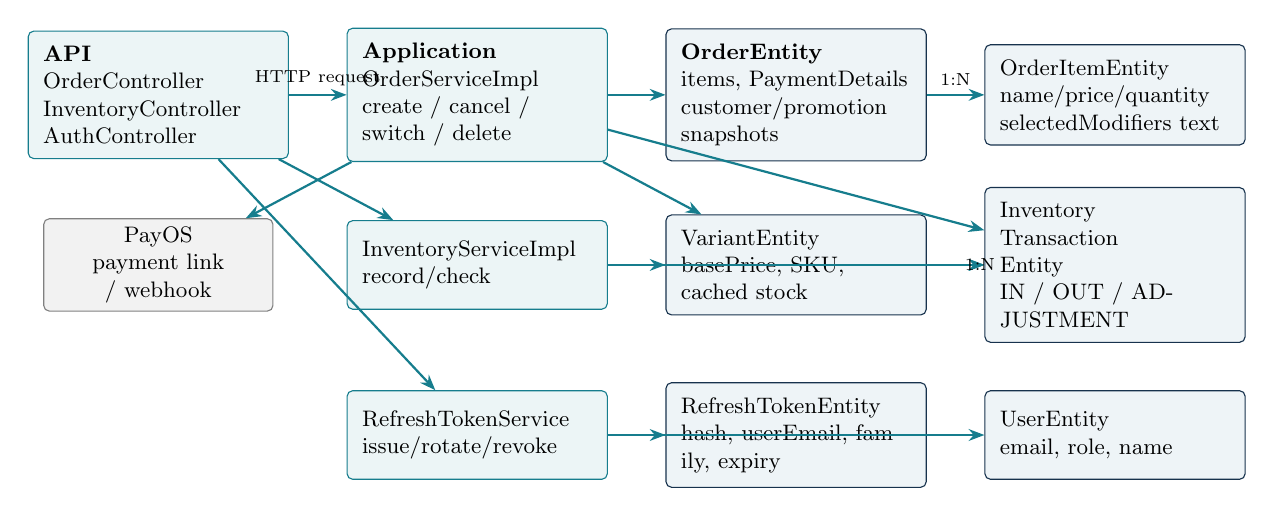
\begin{tikzpicture}[scale=0.9,transform shape,box/.style={draw=navy,rounded corners=2pt,fill=pale,align=left,text width=3.25cm,minimum height=1.25cm,font=\small,inner sep=6pt},svc/.style={draw=teal,rounded corners=2pt,fill=teal!8,align=left,text width=3.25cm,minimum height=1.25cm,font=\small,inner sep=6pt},ext/.style={draw=gray,rounded corners=2pt,fill=gray!10,align=center,text width=3.0cm,minimum height=0.9cm,font=\small},dep/.style={-{Stealth[length=2mm]},draw=teal,thick}]
\node[svc] (api) at (0,4.8) {\textbf{API}\\OrderController\\InventoryController\\AuthController};
\node[svc] (ordersvc) at (4.5,4.8) {\textbf{Application}\\OrderServiceImpl\\create / cancel / switch / delete};
\node[svc] (invsvc) at (4.5,2.4) {InventoryServiceImpl\\record/check};
\node[svc] (authsvc) at (4.5,0) {RefreshTokenService\\issue/rotate/revoke};
\node[box] (order) at (9,4.8) {\textbf{OrderEntity}\\items, PaymentDetails\\customer/promotion snapshots};
\node[box] (item) at (13.5,4.8) {OrderItemEntity\\name/price/quantity\\selectedModifiers text};
\node[box] (stock) at (9,2.4) {VariantEntity\\basePrice, SKU, cached stock};
\node[box] (ledger) at (13.5,2.4) {Inventory\\Transaction\\Entity\\IN / OUT / ADJUSTMENT};
\node[box] (token) at (9,0) {RefreshTokenEntity\\hash, userEmail, family, expiry};
\node[box] (user) at (13.5,0) {UserEntity\\email, role, name};
\node[ext] (payos) at (0,2.4) {PayOS\\payment link / webhook};
\draw[dep] (api) -- node[above,font=\scriptsize]{HTTP request} (ordersvc);
\draw[dep] (api) -- (invsvc);
\draw[dep] (api) -- (authsvc);
\draw[dep] (ordersvc) -- (order);
\draw[dep] (ordersvc) -- (stock);
\draw[dep] (ordersvc) -- (ledger);
\draw[dep] (ordersvc) -- (payos);
\draw[dep] (invsvc) -- (stock);
\draw[dep] (invsvc) -- (ledger);
\draw[dep] (authsvc) -- (token);
\draw[dep] (authsvc) -- (user);
\draw[dep] (order) -- node[above,font=\scriptsize]{1:N} (item);
\draw[dep] (stock) -- node[right,font=\scriptsize]{1:N} (ledger);
\end{tikzpicture}
\caption{Lát cắt lớp chính theo lớp API, application, miền và hệ thống ngoài}
\label{fig:detailed-class-slice}
\end{figure}

\noindent\textbf{Mã Mermaid đầy đủ cho lát cắt lớp:}
\begin{lstlisting}[style=mermaid,caption={Sơ đồ lớp chi tiết ở dạng Mermaid classDiagram},label={lst:class-diagram}]
classDiagram
  class OrderController {
    -orderService: OrderService
    +createOrder(request: OrderRequest): OrderResponse
    +cancelOrder(orderId: String): OrderResponse
    +switchToCash(orderId: String): OrderResponse
    +deleteOrder(orderId: String): void
  }
  class OrderServiceImpl {
    -orderEntityRepository: OrderEntityRepository
    -payOS: PayOS
    -variantRepository: VariantRepository
    -inventoryTransactionRepository: InventoryTransactionRepository
    -promotionService: PromotionService
    -promotionRepository: PromotionRepository
    -customerRepository: CustomerRepository
    -activityLogService: ActivityLogService
    +createOrder(request: OrderRequest): OrderResponse
    +cancelOrder(orderId: String): OrderResponse
    +switchToCash(orderId: String): OrderResponse
    +deleteOrder(orderId: String): void
    -compensatePendingOrder(order: OrderEntity, note: String, reason: String): void
  }
  class InventoryController {
    -inventoryService: InventoryService
    +recordTransaction(request: InventoryTransactionRequest): InventoryTransactionResponse
    +performStockCheck(request: StockCheckRequest): InventoryTransactionResponse
  }
  class InventoryServiceImpl {
    +recordTransaction(request: InventoryTransactionRequest): InventoryTransactionResponse
    +performStockCheck(request: StockCheckRequest): InventoryTransactionResponse
  }
  class AuthController {
    -refreshTokenService: RefreshTokenService
    +login(request: AuthRequest): AuthResponse
    +refresh(rawRefreshToken: String): AuthResponse
    +logout(rawRefreshToken: String): void
  }
  class RefreshTokenService {
    -refreshTokenRepository: RefreshTokenRepository
    -refreshTokenExpirationMs: long
    +issue(userEmail: String): IssuedRefreshToken
    +rotate(rawToken: String): IssuedRefreshToken
    +revoke(rawToken: String): void
  }
  class OrderEntity {
    -id: Long
    -orderId: String
    -customerId: String
    -subtotal: Double
    -grandTotal: Double
    -items: List~OrderItemEntity~
    -paymentDetails: PaymentDetails
    -paymentMethod: PaymentMethod
    +addOrderItem(item: OrderItemEntity): void
  }
  class OrderItemEntity {
    -id: Long
    -itemId: String
    -variantId: String
    -quantity: Integer
    -selectedModifiers: String
    -order: OrderEntity
  }
  class PaymentDetails {
    -orderId: String
    -status: PaymentStatus
    -paymentLinkId: String
    -checkoutUrl: String
    -qrCode: String
  }
  class VariantEntity {
    -variantId: String
    -sku: String
    -basePrice: BigDecimal
    -attributes: Map~String,String~
    -cachedStockQuantity: Integer
  }
  class InventoryTransactionEntity {
    -transactionId: String
    -variant: VariantEntity
    -transactionType: TransactionType
    -quantity: Integer
    -referenceId: String
  }
  class RefreshTokenEntity {
    -tokenHash: String
    -userEmail: String
    -familyId: String
    -issuedAt: Timestamp
    -expiresAt: Timestamp
    -revokedAt: Timestamp
  }
  class UserEntity {
    -userId: String
    -email: String
    -password: String
    -role: String
    -name: String
  }
  class CustomerEntity {
    -customerId: String
    -name: String
    -phoneNumber: String
    -totalSpent: Double
    -orderCount: Integer
    +revertOrderSpending(orderTotal: Double): void
  }
  class PromotionEntity {
    -promotionId: String
    -type: PromotionType
    -discountType: DiscountType
    -discountValue: BigDecimal
    -usageLimit: Integer
    -timesUsed: Integer
  }
  class ActivityLogEntity {
    -logId: String
    -userEmail: String
    -action: String
    -entityType: String
    -entityId: String
    -createdAt: LocalDateTime
  }
  class CategoryEntity
  class ItemEntity
  class ModifierGroupEntity
  class ModifierEntity
  class PaymentWebhookController
  class PayOS
  OrderController ..> OrderServiceImpl
  InventoryController ..> InventoryServiceImpl
  AuthController ..> RefreshTokenService
  OrderServiceImpl --> OrderEntity
  OrderServiceImpl ..> CustomerEntity : lookup by customerId / phone
  OrderServiceImpl ..> PromotionEntity : lookup by promotionId
  OrderEntity "1" *-- "0..*" OrderItemEntity
  OrderEntity *-- PaymentDetails : embedded
  VariantEntity "1" <-- "0..*" InventoryTransactionEntity
  ItemEntity "1" --> "0..*" VariantEntity
  CategoryEntity "1" --> "0..*" ItemEntity
  ItemEntity "0..*" --> "0..*" ModifierGroupEntity : join table
  ModifierGroupEntity "1" --> "0..*" ModifierEntity
  RefreshTokenService --> RefreshTokenEntity
  UserEntity .. RefreshTokenEntity : scalar email, no FK
  UserEntity .. ActivityLogEntity : scalar email, no FK
  PaymentWebhookController ..> PayOS
  PaymentWebhookController ..> OrderEntity
\end{lstlisting}

\section{Từ điển dữ liệu các lớp miền}
Các bảng sau ghi kiểu dữ liệu Java và visibility khai báo. Cột quan hệ mang kiểu entity/danh sách thay cho kiểu SQL. Mọi trường được liệt kê là private trong mã nguồn; Lombok sinh accessor tùy annotation, còn các thao tác public quan trọng được phân tích ở mục 3.4. Giá trị mặc định được ghi khi có ý nghĩa nghiệp vụ.

\subsection{Danh mục và cấu hình hàng bán}
\ClassTableTitle{CategoryEntity — danh mục}
\small\begin{longtable}{@{}D{3.25cm}D{3.35cm}D{1.35cm}D{6.75cm}@{}}\toprule Thuộc tính & Kiểu Java & Phạm vi & Ý nghĩa\\\midrule\endfirsthead\toprule Thuộc tính & Kiểu Java & Phạm vi & Ý nghĩa\\\midrule\endhead\bottomrule\endfoot
id & Long & private & Khóa nội bộ tự tăng.\\categoryId & String & private & Mã danh mục nghiệp vụ; có unique index nhưng migration cho phép NULL.\\name & String & private & Tên danh mục; unique index ở DB, nullable theo migration.\\description & String & private & Mô tả.\\bgColor & String & private & Mã/mô tả màu nền giao diện.\\imgUrl & String & private & URL ảnh danh mục.\\createdAt & Timestamp & private & Thời điểm tạo.\\updatedAt & Timestamp & private & Thời điểm cập nhật.\\\end{longtable}\normalsize

\ClassTableTitle{ItemEntity — mặt hàng cha}
\small\begin{longtable}{@{}D{3.25cm}D{3.35cm}D{1.35cm}D{6.75cm}@{}}\toprule Thuộc tính & Kiểu Java & Phạm vi & Ý nghĩa\\\midrule\endfirsthead\toprule Thuộc tính & Kiểu Java & Phạm vi & Ý nghĩa\\\midrule\endhead\bottomrule\endfoot
id & Long & private & Khóa nội bộ.\\itemId & String & private & Mã mặt hàng nghiệp vụ, unique ở migration nhưng cho phép NULL trong schema.\\name & String & private & Tên hiển thị.\\description & String & private & Nội dung mô tả.\\price & BigDecimal & private & Giá ở cấp Item; trường hiện diện cùng giá basePrice của Variant.\allowbreak \\createdAt / updatedAt & Timestamp & private & Mốc tạo/cập nhật.\\imgUrl & String & private & URL ảnh.\\category & CategoryEntity & private & Quan hệ ManyToOne tới Category.\allowbreak \\variants & List\textless VariantEntity\textgreater & private & Tập biến thể; quan hệ OneToMany, cascade theo mapping.\\modifierGroups & List\textless\allowbreak ModifierGroupEntity\textgreater & private & Tập nhóm modifier; quan hệ ManyToMany qua bảng nối.\\\end{longtable}\normalsize

\ClassTableTitle{VariantEntity — biến thể/SKU}
\small\begin{longtable}{@{}D{3.25cm}D{3.35cm}D{1.35cm}D{6.75cm}@{}}\toprule Thuộc tính & Kiểu Java & Phạm vi & Ý nghĩa\\\midrule\endfirsthead\toprule Thuộc tính & Kiểu Java & Phạm vi & Ý nghĩa\\\midrule\endhead\bottomrule\endfoot
id & Long & private & Khóa nội bộ.\\variantId & String & private & Mã biến thể duy nhất.\\sku & String & private & Mã SKU duy nhất.\\basePrice & BigDecimal & private & Giá cơ sở; được dùng để chụp giá dòng hàng.\\attributes & Map\textless String, String\textgreater & private & Thuộc tính biến thể động; converter lưu ở cột TEXT.\\cachedStockQuantity & Integer & private & Bản cache tổng ledger; có thể âm theo quy tắc chấp nhận bán khi thiếu hàng.\\item & ItemEntity & private & Quan hệ ManyToOne tới Item.\allowbreak \\createdAt / updatedAt & Timestamp & private & Mốc tạo/cập nhật.\\\end{longtable}\normalsize

\ClassTableTitle{ModifierGroupEntity và ModifierEntity — nhóm/tùy chọn thêm}
\small\begin{longtable}{@{}D{3.25cm}D{3.35cm}D{1.35cm}D{6.75cm}@{}}\toprule Lớp.thuộc tính & Kiểu Java & Phạm vi & Ý nghĩa\\\midrule\endfirsthead\toprule Lớp.thuộc tính & Kiểu Java & Phạm vi & Ý nghĩa\\\midrule\endhead\bottomrule\endfoot
Group.\allowbreak id & Long & private & Khóa nội bộ nhóm.\\Group.\allowbreak groupId & String & private & Mã nhóm duy nhất.\\Group.\allowbreak name / description & String & private & Tên bắt buộc trong migration và mô tả tùy chọn.\\Group.\allowbreak minSelections / maxSelections & Integer & private & Số lựa chọn tối thiểu/tối đa; mặc định lần lượt 0 và 1.\\Group.\allowbreak modifiers & List\textless ModifierEntity\textgreater & private & Tập tùy chọn thuộc nhóm.\\Group.\allowbreak items & List\textless ItemEntity\textgreater & private & Tập Item liên kết qua bảng nối.\\Group.\allowbreak createdAt / updatedAt & Timestamp & private & Mốc tạo/cập nhật.\\Modifier.\allowbreak id & Long & private & Khóa nội bộ tùy chọn.\\Modifier.\allowbreak modifierId & String & private & Mã modifier duy nhất.\\Modifier.\allowbreak name & String & private & Tên tùy chọn.\\Modifier.\allowbreak priceAdjustment & BigDecimal & private & Phần cộng/trừ giá, mặc định BigDecimal.ZERO.\\Modifier.\allowbreak modifierGroup & ModifierGroupEntity & private & Quan hệ ManyToOne về nhóm.\\Modifier.\allowbreak createdAt / updatedAt & Timestamp & private & Mốc tạo/cập nhật.\\\end{longtable}\normalsize

\subsection{Bán hàng, khách hàng và khuyến mãi}
\ClassTableTitle{OrderEntity — đơn hàng}
\small\begin{longtable}{@{}D{3.25cm}D{3.35cm}D{1.35cm}D{6.75cm}@{}}\toprule Thuộc tính & Kiểu Java & Phạm vi & Ý nghĩa\\\midrule\endfirsthead\toprule Thuộc tính & Kiểu Java & Phạm vi & Ý nghĩa\\\midrule\endhead\bottomrule\endfoot
id & Long & private & PK số; đồng thời dùng làm orderCode khi tạo yêu cầu PayOS.\\orderId & String & private & Mã đơn nghiệp vụ \texttt{ORD...}; cột order\_code unique NOT NULL.\\customerId / customerName / phoneNumber & String & private & Mã và snapshot khách hàng; không có relation/FK tới Customer.\allowbreak \\subtotal / discountAmount / tax / grandTotal & Double & private & Tổng tiền; discountAmount mặc định 0.0.\\promotionId / promotionName & String & private & Mã/tên promotion snapshot.\\createdAt & LocalDateTime & private & Thời điểm tạo; gán ở callback PrePersist.\\items & List\textless OrderItemEntity\textgreater & private & Danh sách dòng; OneToMany cascade ALL, orphanRemoval=true.\\paymentDetails & PaymentDetails & private & Giá trị embeddable gồm trạng thái, link và QR.\\paymentMethod & PaymentMethod & private & Enum CASH hoặc PAYOS; lưu dạng chuỗi.\\\end{longtable}\normalsize

\ClassTableTitle{OrderItemEntity và PaymentDetails — dòng đơn và trạng thái thanh toán}
\small\begin{longtable}{@{}D{3.25cm}D{3.35cm}D{1.35cm}D{6.75cm}@{}}\toprule Lớp.thuộc tính & Kiểu Java & Phạm vi & Ý nghĩa\\\midrule\endfirsthead\toprule Lớp.thuộc tính & Kiểu Java & Phạm vi & Ý nghĩa\\\midrule\endhead\bottomrule\endfoot
OrderItem.\allowbreak id & Long & private & Khóa dòng tự tăng.\\OrderItem.\allowbreak itemId / variantId & String & private & Mã mặt hàng/biến thể dạng snapshot scalar; không có FK.\\OrderItem.\allowbreak name & String & private & Tên hàng tại thời điểm bán.\\OrderItem.\allowbreak basePrice / price & Double & private & Giá cơ sở và giá dòng tại thời điểm bán.\\OrderItem.\allowbreak quantity & Integer & private & Số lượng dòng; cột migration nullable, không có CHECK.\\OrderItem.\allowbreak selectedModifiers & String & private & Nội dung tùy chọn được lưu vào cột TEXT.\\OrderItem.\allowbreak order & OrderEntity & private & ManyToOne tới đơn, cột order\_id là FK.\\Payment.\allowbreak orderId & String & private & Mã PayOS/domain được đặt bởi service.\\Payment.\allowbreak status & PaymentStatus & private & PENDING / COMPLETED / FAILED / CANCELLED; cột migration TINYINT ordinal.\\Payment.\allowbreak paymentLinkId & String & private & Định danh payment link.\\Payment.\allowbreak checkoutUrl & String & private & URL thanh toán, độ dài cột 1000.\\Payment.\allowbreak qrCode & String & private & Dữ liệu QR, cột TEXT.\\\end{longtable}\normalsize

\ClassTableTitle{CustomerEntity và PromotionEntity — CRM/khuyến mãi}
\small\begin{longtable}{@{}D{3.25cm}D{3.35cm}D{1.35cm}D{6.75cm}@{}}\toprule Lớp.thuộc tính & Kiểu Java & Phạm vi & Ý nghĩa\\\midrule\endfirsthead\toprule Lớp.thuộc tính & Kiểu Java & Phạm vi & Ý nghĩa\\\midrule\endhead\bottomrule\endfoot
Customer.\allowbreak id & Long & private & Khóa nội bộ.\\Customer.\allowbreak customerId & String & private & Mã khách hàng duy nhất, NOT NULL trong migration.\\Customer.\allowbreak name / phoneNumber & String & private & Tên và điện thoại; phoneNumber unique, NOT NULL.\\Customer.\allowbreak email & String & private & Email tùy chọn.\\Customer.\allowbreak totalSpent & Double & private & Tổng tiền tích lũy; mặc định 0.0, cập nhật khi tạo/hủy đơn.\\Customer.\allowbreak orderCount & Integer & private & Số đơn tích lũy; mặc định 0.\\Customer.\allowbreak createdAt / updatedAt & Timestamp & private & Mốc tạo/cập nhật tự động.\\Promotion.\allowbreak id / promotionId & Long / String & private & Khóa nội bộ và mã promotion duy nhất.\\Promotion.\allowbreak name / description & String & private & Tên bắt buộc và mô tả tùy chọn.\\Promotion.\allowbreak type / discountType & PromotionType / DiscountType & private & Phân loại promotion và cách tính giảm.\\Promotion.\allowbreak code & String & private & Coupon code tùy chọn, unique index ở DB nhưng cho phép NULL.\\Promotion.\allowbreak discountValue / maxDiscountAmount & BigDecimal & private & Giá trị giảm và trần giảm tùy chọn.\\Promotion.\allowbreak minOrderAmount & BigDecimal & private & Giá trị đơn tối thiểu, mặc định ZERO.\\Promotion.\allowbreak startDate / endDate & LocalDate & private & Khoảng ngày hiệu lực.\\Promotion.\allowbreak startTime / endTime & LocalTime & private & Khoảng giờ hiệu lực.\\Promotion.\allowbreak daysOfWeek & String & private & Chuỗi ngày áp dụng, không phải bảng nối ngày.\\Promotion.\allowbreak buyVariantId / getVariantId & String & private & Mã biến thể cho khuyến mãi dạng mua/tặng.\\Promotion.\allowbreak bogoDiscountPercent & BigDecimal & private & Phần trăm giảm ở nhánh BOGO, mặc định 100.\\Promotion.\allowbreak usageLimit / timesUsed & Integer & private & Giới hạn và bộ đếm lượt dùng.\\Promotion.\allowbreak isActive & Boolean & private & Cờ kích hoạt, mặc định true.\\Promotion.\allowbreak createdAt / updatedAt & Timestamp & private & Mốc tạo/cập nhật.\\\end{longtable}\normalsize

\subsection{Kho, định danh và kiểm toán}
\ClassTableTitle{InventoryTransactionEntity và RefreshTokenEntity}
\small\begin{longtable}{@{}D{3.25cm}D{3.35cm}D{1.35cm}D{6.75cm}@{}}\toprule Lớp.thuộc tính & Kiểu Java & Phạm vi & Ý nghĩa\\\midrule\endfirsthead\toprule Lớp.thuộc tính & Kiểu Java & Phạm vi & Ý nghĩa\\\midrule\endhead\bottomrule\endfoot
InventoryTx.\allowbreak id & Long & private & PK nội bộ.\\InventoryTx.\allowbreak transactionId & String & private & Mã transaction duy nhất, NOT NULL.\\InventoryTx.\allowbreak variant & VariantEntity & private & ManyToOne, FK variant\_id bắt buộc; ON DELETE CASCADE.\\InventoryTx.\allowbreak transactionType & TransactionType & private & IN, OUT hoặc ADJUSTMENT, lưu enum dạng String.\\InventoryTx.\allowbreak quantity & Integer & private & Lượng có dấu: IN dương, OUT âm, ADJUSTMENT chênh lệch.\\InventoryTx.\allowbreak referenceId / note & String & private & Tham chiếu nghiệp vụ và ghi chú.\\InventoryTx.\allowbreak createdAt & Timestamp & private & Thời điểm tạo, Hibernate gán.\\RefreshToken.\allowbreak id & Long & private & PK nội bộ tự tăng.\\RefreshToken.\allowbreak tokenHash & String & private & SHA-256 digest Base64 URL-safe; unique NOT NULL.\\RefreshToken.\allowbreak userEmail & String & private & Email tài khoản; NOT NULL nhưng migration không tạo FK user.\\RefreshToken.\allowbreak familyId & String & private & Định danh family; có index tra cứu.\\RefreshToken.\allowbreak issuedAt / expiresAt & Timestamp & private & Thời điểm phát hành và hết hạn.\\RefreshToken.\allowbreak revokedAt & Timestamp & private & Thời điểm thu hồi; NULL nghĩa là chưa bị thu hồi.\\\end{longtable}\normalsize

\ClassTableTitle{UserEntity và ActivityLogEntity}
\small\begin{longtable}{@{}D{3.25cm}D{3.35cm}D{1.35cm}D{6.75cm}@{}}\toprule Lớp.thuộc tính & Kiểu Java & Phạm vi & Ý nghĩa\\\midrule\endfirsthead\toprule Lớp.thuộc tính & Kiểu Java & Phạm vi & Ý nghĩa\\\midrule\endhead\bottomrule\endfoot
User.\allowbreak id & Long & private & PK nội bộ.\\User.\allowbreak userId / email & String & private & Mã tài khoản và email; unique index trong migration.\\User.\allowbreak password & String & private & Chuỗi xác thực đã qua encoder khi tạo/lưu tài khoản.\\User.\allowbreak role & String & private & Authority dùng cho phân quyền.\\User.\allowbreak name & String & private & Tên hiển thị trong AuthResponse/UI.\\User.\allowbreak createdAt / updatedAt & Timestamp & private & Mốc tạo/cập nhật.\\ActivityLog.\allowbreak id & Long & private & PK nội bộ.\\ActivityLog.\allowbreak logId & String & private & Mã nhật ký unique NOT NULL.\\ActivityLog.\allowbreak userEmail & String & private & Email người thao tác, NOT NULL, không có FK.\\ActivityLog.\allowbreak action & String & private & Hành động như LOGIN / CREATE / UPDATE / DELETE / CANCEL.\\ActivityLog.\allowbreak entityType / entityId & String & private & Loại đối tượng và business ID liên quan.\\ActivityLog.\allowbreak description & String & private & Mô tả tóm tắt, tối đa 1000 ký tự theo migration.\\ActivityLog.\allowbreak createdAt & LocalDateTime & private & Thời điểm ghi log, NOT NULL.\\\end{longtable}\normalsize

\subsection{Các lớp điều phối trong sơ đồ}
\begin{table}[htbp]
\centering\small
\caption{Thuộc tính phụ thuộc và trách nhiệm của các lớp application/API}
\begin{tabularx}{\textwidth}{@{}p{3.3cm}p{5.8cm}Y@{}}\toprule
Lớp & Thuộc tính khai báo (đều private) & Phương thức công khai trọng tâm\\\midrule
OrderController & \texttt{OrderService orderService} & GET danh sách/phân trang; POST tạo; DELETE; GET latest/by id; POST cancel/switch-to-cash.\\
OrderServiceImpl & repository Order; PayOS; VariantRepository; InventoryTransactionRepository; PromotionService/Repository; CustomerRepository; ActivityLogService; ObjectMapper. & createOrder, cancelOrder, switchToCash, deleteOrder, getOrdersPaginated.\\
InventoryController & \texttt{InventoryService inventoryService} & POST ghi giao dịch/kiểm kê; GET toàn bộ và theo Variant.\\
InventoryServiceImpl & InventoryTransactionRepository, VariantRepository & recordTransaction, performStockCheck, getTransactionsByVariant.\\
AuthController & PasswordEncoder, AuthenticationManager, AppUserDetailsService, UserService, JwtUtil, ActivityLogService, RefreshTokenService; cấu hình cookie/TTL. & login, refresh, logout; helper authenticate và cookie private.\\
RefreshTokenService & RefreshTokenRepository, SecureRandom, refreshTokenExpirationMs & issue, rotate, revoke; hash và phát raw token là helper private.\\
PaymentWebhook\allowbreak Controller & PayOS, OrderEntityRepository & handleWebhook(Webhook): xác minh callback, cập nhật trạng thái thành COMPLETED khi code=00.\\
Repository ports & Không có state instance nghiệp vụ riêng trong interface; khai báo truy vấn Spring Data/JPA. & Tra cứu theo mã/email, lưu entity, khóa token khi rotate, tổng hợp stock ledger.\\
\bottomrule\end{tabularx}
\end{table}
\section{Đặc tả chi tiết các phương thức trọng tâm}
Các hợp đồng dưới đây mô tả chữ ký và hiệu ứng trực tiếp của lớp service. Tiền điều kiện được chia thành điều kiện do route/service kiểm tra và điều kiện môi trường. Nếu mã nguồn không kiểm tra một điều kiện, báo cáo ghi “không được kiểm tra tường minh” thay vì biến nó thành yêu cầu đã triển khai. Transactional annotation chỉ bảo đảm phạm vi giao dịch cơ sở dữ liệu trong ứng dụng; không làm cho thao tác với PayOS trở thành giao dịch phân tán.

\subsection{OrderServiceImpl.createOrder}
\begin{table}[htbp]
\centering\small
\caption{Hợp đồng phương thức createOrder}
\begin{tabularx}{\textwidth}{@{}p{3.1cm}Y@{}}\toprule
Thành phần & Đặc tả\\\midrule
Chữ ký & \texttt{createOrder(request: OrderRequest): OrderResponse}; public, \texttt{@Transactional}.\\
Input & OrderRequest gồm customerId/customerName/phoneNumber, cartItems, couponCode, appliedPromotionId và paymentMethod. Mỗi OrderItemRequest gồm itemId, variantId, name, basePrice, price, quantity, selectedModifiers. Các tổng client gửi không phải nguồn cuối: service thay bằng kết quả evaluatePromotion.\\
Output & OrderResponse đã ánh xạ từ OrderEntity mới lưu, gồm trạng thái, tổng tiền, dòng đơn và PaymentDetails khi có.\\
Tiền điều kiện & Request đã được JSON deserialize; người gọi đã qua security filter. Service không có kiểm tra tường minh giỏ hàng khác null/không rỗng, số lượng dương, giá client hợp lệ hoặc đủ tồn kho tại entry point. Hợp đồng bên trong phụ thuộc PromotionService.evaluatePromotion và kiểu paymentMethod hợp lệ.\\
Hậu điều kiện & Lưu Order cùng các dòng; cập nhật số liệu khách hàng/promotion nếu tìm thấy; ghi OUT cho Variant phân giải được; tái tính cached stock; với PAYOS tạo và lưu payment link. Với CASH trạng thái ban đầu là COMPLETED, còn phương thức khác được đặt PENDING theo nhánh hiện tại.\\
Lỗi/ngoại lệ & Đạt quota promotion giữa lúc đánh giá và lúc ghi nhận: HTTP 400. Lỗi PayOS: RuntimeException. Lỗi DB/ánh xạ: transaction ứng dụng thất bại. Không tìm được Variant cho dòng không làm toàn bộ request bị từ chối trong phần xử lý stock quan sát được.\\
\bottomrule\end{tabularx}
\end{table}

\textbf{Thuật toán quan sát được:}
\begin{lstlisting}[style=pseudo]
function createOrder(request):
    cartForEvaluation = map request.cartItems to EvaluationCartItem
    evaluation = promotionService.evaluatePromotion(couponCode, cartForEvaluation)
    order = map request to OrderEntity
    order.subtotal       = evaluation.subtotal
    order.discountAmount = evaluation.discountAmount
    order.tax            = evaluation.tax
    order.grandTotal     = evaluation.grandTotal
    order.promotion      = evaluation.appliedPromotion

    customer = find by trimmed customerId
    if customer is absent and phone is nonblank and phone != "0000000000":
        customer = find by trimmed phone
    if customer exists:
        copy customer snapshot to order
        increment customer.orderCount and totalSpent by grandTotal
        persist customer
    else:
        set fallback customer name/phone when absent

    if an applied promotion exists:
        reload promotion
        if usageLimit reached: reject with BAD_REQUEST
        increment timesUsed and persist

    set payment status: CASH -> COMPLETED, otherwise -> PENDING
    map cart items; attach each item to order; persist order
    for each saved line:
        variant = find by variantId, else first variant for itemId
        if variant exists:
            append OUT transaction with quantity = -abs(line.quantity or 1)
            cachedStock = sum(ledger quantities for variant)
    if payment method is PAYOS:
        create payment link using order database id as orderCode
        save link id, checkout URL and QR data
    attempt CREATE activity log
    return mapped OrderResponse
\end{lstlisting}

Một hệ quả nghiệp vụ quan trọng là sổ kho được cập nhật khi tạo đơn, trước khi webhook báo thanh toán thành công. Đơn PENDING do đó đã giữ chỗ bằng cách trừ tồn. Nhánh hủy phải bù IN; nhánh đổi sang CASH không trừ lần nữa. Không có bước kiểm tra số dư tồn trước OUT, phù hợp với quy tắc cho phép tồn âm trong ADR 0002 nhưng không chứng minh ứng dụng thực hiện đồng bộ offline.

\subsection{OrderServiceImpl.cancelOrder và compensatePendingOrder}
\begin{table}[htbp]
\centering\small
\caption{Hợp đồng hủy đơn và bù trừ}
\begin{tabularx}{\textwidth}{@{}p{3.1cm}Y@{}}\toprule
Thành phần & Đặc tả\\\midrule
Chữ ký public & \texttt{cancelOrder(orderId: String): OrderResponse}; public, transactional.\\
Chữ ký helper & \texttt{compensatePendingOrder(order: OrderEntity, ledgerNotePrefix: String, payosCancelReason: String): void}; private.\\
Input & Mã đơn nghiệp vụ. Helper nhận entity đã nạp cùng nội dung ghi chú và lý do hủy liên kết PayOS.\\
Output & OrderResponse ở trạng thái CANCELLED; helper không trả giá trị.\\
Tiền điều kiện & Tìm thấy đơn; PaymentDetails khác null; PaymentStatus đúng PENDING.\\
Hậu điều kiện & Trạng thái local thành CANCELLED; ghi IN cho từng Variant tìm được; cache kho tính lại; hoàn bộ đếm promotion nếu lớn hơn 0; gọi Customer.revertOrderSpending khi Customer còn tồn tại; yêu cầu PayOS hủy link; lưu đơn và log CANCEL.\\
Lỗi/ngoại lệ & Không tìm thấy đơn: 404. Không có PaymentDetails/PENDING: 400. Lỗi remote PayOS bị catch và chỉ ghi warning, nên hậu điều kiện “PayOS đã hủy” không được bảo đảm.\\
\bottomrule\end{tabularx}
\end{table}

\begin{lstlisting}[style=pseudo]
function cancelOrder(orderId):
    order = findByOrderId(orderId) or NOT_FOUND
    if order.paymentDetails is absent or status != PENDING:
        reject BAD_REQUEST
    order.paymentDetails.status = CANCELLED
    compensatePendingOrder(order, cancellation note, PayOS reason)
    save order
    attempt CANCEL activity log
    return order response

function compensatePendingOrder(order, notePrefix, reason):
    for each line in order.items:
        variant = find by line.variantId, else first variant for line.itemId
        if variant exists:
            append IN transaction with quantity = abs(line.quantity or 1)
            recalculate variant cached stock from ledger
    if order has promotionId:
        if promotion exists and timesUsed > 0: decrement and save
    if order has customerId and customer exists:
        revert customer orderCount/totalSpent and save
    if order.paymentMethod == PAYOS:
        try cancel remote payment link; catch exception and log warning
\end{lstlisting}

\subsection{OrderServiceImpl.deleteOrder}
\begin{table}[htbp]
\centering\small
\caption{Hợp đồng xóa đơn}
\begin{tabularx}{\textwidth}{@{}p{3.1cm}Y@{}}\toprule
Thành phần & Đặc tả\\\midrule
Chữ ký & \texttt{deleteOrder(orderId: String): void}; public, transactional; controller trả HTTP 204 nếu không có lỗi.\\
Input / output & orderId dạng String; không có body kết quả.\\
Tiền điều kiện & Order tồn tại; PaymentDetails có thể null nhưng trạng thái null/khác PENDING-CANCELLED sẽ bị từ chối.\\
Hậu điều kiện & PENDING: bù trừ trước khi xóa. CANCELLED: không bù lần hai. Xóa Order dẫn đến xóa OrderItem bằng cascade JPA/ON DELETE CASCADE; log DELETE được gọi sau thao tác xóa.\\
Lỗi/ngoại lệ & Không tìm thấy: 404. COMPLETED: HTTP 400 với thông điệp bảo vệ lịch sử kế toán. FAILED/null/trạng thái khác: HTTP 400. Lỗi từ DB làm transaction thất bại.\\
\bottomrule\end{tabularx}
\end{table}

Đây là invariant được cưỡng chế trong service, không phải constraint ở tầng bảng. Một lệnh SQL trực tiếp ngoài application vẫn có thể xóa đơn COMPLETED nếu tài khoản DB cho phép. Nhận định này phân biệt quy tắc ứng dụng với bất biến vật lý.

\subsection{OrderServiceImpl.switchToCash}
\begin{table}[htbp]
\centering\small
\caption{Hợp đồng chuyển PENDING QR sang tiền mặt}
\begin{tabularx}{\textwidth}{@{}p{3.1cm}Y@{}}\toprule
Thành phần & Đặc tả\\\midrule
Chữ ký & \texttt{switchToCash(orderId: String): OrderResponse}; public, transactional.\\
Tiền điều kiện & Order tồn tại, có PaymentDetails và đang PENDING.\\
Hậu điều kiện & Nếu method cũ là PAYOS thì gọi hủy link; đổi paymentMethod CASH, status COMPLETED; lưu và log UPDATE. Không ghi giao dịch kho mới.\\
Ngoại lệ & Không tìm thấy: 404; trạng thái hoặc payment details không đúng: 400. Helper bắt lỗi hủy PayOS và tiếp tục cập nhật local.\\
Ràng buộc & Giữ số lượng đã trừ, promotion và CRM đã ghi khi tạo đơn; tránh hoàn rồi trừ lại làm phát sinh bù trừ lặp. Kết quả remote cancel không được xác nhận trong response.\\
\bottomrule\end{tabularx}
\end{table}

\subsection{InventoryServiceImpl.recordTransaction}
\begin{table}[htbp]
\centering\small
\caption{Hợp đồng ghi giao dịch tồn kho}
\begin{tabularx}{\textwidth}{@{}p{3.1cm}Y@{}}\toprule
Thành phần & Đặc tả\\\midrule
Chữ ký & \texttt{recordTransaction(request: InventoryTransactionRequest): InventoryTransactionResponse}; public, transactional.\\
Input & variantId: String; quantity: Integer; transactionType: TransactionType; referenceId/note tùy chọn.\\
Output & Response gồm transaction đã lưu và cached stock mới.\\
Tiền điều kiện & variantId không trống; quantity khác null và lớn hơn 0; transactionType khác null; Variant tồn tại.\\
Hậu điều kiện & IN lượng dương; OUT lượng âm theo \texttt{-abs(quantity)}; ADJUSTMENT giữ quantity gửi vào. Lưu/flush ledger, sum ledger theo Variant, cập nhật cachedStockQuantity.\\
Ngoại lệ & Thiếu ID/type hoặc quantity không hợp lệ: 400. Không thấy Variant: 404.\\
\bottomrule\end{tabularx}
\end{table}

\begin{lstlisting}[style=pseudo]
function recordTransaction(request):
    require nonblank request.variantId
    require request.quantity > 0
    require request.transactionType exists
    variant = findVariant(request.variantId) or NOT_FOUND
    if type == IN: signedQuantity = abs(quantity)
    else if type == OUT: signedQuantity = -abs(quantity)
    else: signedQuantity = quantity
    tx = saveAndFlush(variant, type, signedQuantity, referenceId, note)
    stock = sumLedger(variant.variantId)
    variant.cachedStockQuantity = stock or 0
    save variant
    return response(tx, variant.cachedStockQuantity)
\end{lstlisting}

Với API ghi giao dịch thủ công, quantity đầu vào bắt buộc lớn hơn 0 nên ADJUSTMENT trực tiếp qua route này không thể giảm tồn bằng số âm. API kiểm kê ở mục sau tạo discrepancy âm từ actualCount-currentStock. Đây là khác biệt giữa hai đường ghi dữ liệu; không nên gộp cả hai thành một quy tắc đầu vào duy nhất.

\subsection{InventoryServiceImpl.performStockCheck}
\begin{table}[htbp]
\centering\small
\caption{Hợp đồng kiểm kê và điều chỉnh chênh lệch}
\begin{tabularx}{\textwidth}{@{}p{3.1cm}Y@{}}\toprule
Thành phần & Đặc tả\\\midrule
Chữ ký & \texttt{performStockCheck(request: StockCheckRequest): InventoryTransactionResponse}; public, transactional.\\
Input & variantId: String; actualCount: Integer; referenceId/note tùy chọn.\\
Output & Bản ghi ADJUSTMENT và cached stock sau khi tái tính.\\
Tiền điều kiện & variantId không trống; actualCount khác null và không âm; Variant tồn tại.\\
Hậu điều kiện & discrepancy = actualCount - cachedStock (null coi như 0); ghi ADJUSTMENT với lượng discrepancy. Nếu không truyền ref, sinh \texttt{CHECK-...}; nếu không có note thì tạo ghi chú khớp/chênh lệch. Lưu và tính lại ledger/cache.\\
Ngoại lệ & ID thiếu hoặc actualCount âm: 400. Variant không tồn tại: 404.\\
Ràng buộc & discrepancy có thể âm hoặc bằng 0; không được áp ràng buộc quantity $> 0$ cho bảng ledger nếu muốn bảo toàn kiểm kê/xuất kho.\\
\bottomrule\end{tabularx}
\end{table}

\subsection{RefreshTokenService.rotate}
\begin{table}[htbp]
\centering\small
\caption{Hợp đồng xoay refresh token}
\begin{tabularx}{\textwidth}{@{}p{3.1cm}Y@{}}\toprule
Thành phần & Đặc tả\\\midrule
Chữ ký & \texttt{rotate(rawToken: String): IssuedRefreshToken}; public, transactional.\\
Input / output & Raw token từ cookie; trả token mới, hạn dùng và userEmail cho AuthController. Raw token mới chỉ trả qua object nội bộ/cookie; DB lưu digest.\\
Tiền điều kiện & Token không null/trống; SHA-256 hash trùng tokenHash trong DB; bản ghi chưa revoke và expiresAt còn sau thời điểm hiện tại.\\
Hậu điều kiện dự kiến & Thu hồi token cũ và phát token mới trong cùng family, lưu hash/hạn mới.\\
Lỗi/ngoại lệ & Thiếu/sai/hết hạn/revoked: ResponseStatusException không xác thực được. Replay gọi revokeActiveByFamilyId rồi ném lỗi. Vì method transactional và lỗi là unchecked, theo quy tắc rollback mặc định của Spring, cần xác minh thao tác thu hồi family có được commit hay bị rollback; mã nguồn được khảo sát không cho thấy noRollbackFor hoặc transaction riêng \cite{springtx}.\\
Ràng buộc & Hành vi “thu hồi cả family sau replay” là ý định thể hiện bằng lệnh repository; không báo cáo như kết quả bền vững đã được kiểm chứng.\\
\bottomrule\end{tabularx}
\end{table}

\begin{lstlisting}[style=pseudo]
function rotate(rawToken):
    if rawToken is null or blank: reject INVALID_TOKEN
    existing = findByHashForUpdate(SHA256(rawToken)) or INVALID_TOKEN
    now = currentTimestamp()
    if existing.revokedAt is not null:
        request revocation of every active token in existing.familyId
        reject INVALID_TOKEN
    if existing.expiresAt <= now:
        existing.revokedAt = now
        save existing
        reject INVALID_TOKEN
    existing.revokedAt = now
    save existing
    return issue(existing.userEmail, existing.familyId)
\end{lstlisting}

\noindent Tài liệu Spring mô tả rollback mặc định cho unchecked exceptions trong giao dịch khai báo \cite{springtx}. Do nhánh replay vừa thay đổi family vừa ném unchecked exception trong cùng phương thức transactional, đây là điểm cần xử lý/kiểm chứng riêng nếu yêu cầu bảo mật bắt buộc thu hồi family phải được bảo đảm. Báo cáo không biến “đã gọi câu lệnh UPDATE” thành “đã commit thành công”.

\section{Máy trạng thái đơn hàng và bất biến xuyên phân hệ}
\begin{table}[htbp]
\centering\small
\caption{Chuyển trạng thái Order quan sát được}
\begin{tabularx}{\textwidth}{@{}p{2.8cm}p{3.3cm}p{5.2cm}Y@{}}\toprule
Trạng thái ban đầu & Sự kiện & Trạng thái kế tiếp & Hiệu ứng kèm theo\\\midrule
Mới tạo, CASH & createOrder & COMPLETED & Ledger OUT đã ghi; CRM/promotion cập nhật; không tạo PayOS link.\\
Mới tạo, PAYOS & createOrder & PENDING & Ledger OUT đã ghi; PayOS link/QR lưu sau khi tạo link.\\
PENDING & webhook code=00 & COMPLETED & Cập nhật status thanh toán; không thấy kiểm tra transition/idempotency tường minh.\\
PENDING & cancelOrder & CANCELLED & Ledger IN bù trừ; hoàn promotion/CRM; thử hủy PayOS.\\
PENDING/PAYOS & switchToCash & COMPLETED/CASH & Thử hủy link, giữ lần OUT ban đầu.\\
PENDING & deleteOrder & Đã xóa & Bù trừ trước khi xóa.\\
CANCELLED & deleteOrder & Đã xóa & Không bù trừ lặp.\\
COMPLETED & deleteOrder & Không đổi & Bị từ chối tại service.\\
\bottomrule\end{tabularx}
\end{table}

Một số bất biến nghiệp vụ có thể phát biểu bằng ngôn ngữ đặc tả như sau: (i) tổng tiền dùng trong đơn phải lấy từ kết quả tính tại máy chủ; (ii) mỗi lần hủy PENDING chỉ được bù trừ một lần; (iii) chuyển QR sang CASH không phát sinh giao dịch kho OUT lần hai; (iv) completed order không xóa qua service; (v) cached stock bằng tổng signed quantity của ledger tại thời điểm tái tính; (vi) các quan hệ ID dạng snapshot không được xem là FK; (vii) PayOS và DB là hai ranh giới giao dịch khác nhau; (viii) ghi activity log hiện là best-effort vì lỗi ghi bị hấp thụ trong service.

\chapter{SƠ ĐỒ QUAN HỆ THỰC THỂ — ERD}

\section{ERD vật lý theo migration hiện hành}
Migration \texttt{V1\_\_init\_schema.sql} tạo \textbf{14 bảng} InnoDB. Sơ đồ sau phản ánh FK được khai báo thật; nó không bổ sung đường nối chỉ vì hai bảng chứa mã có tên tương tự. Một số bảng như \texttt{tbl\_orders}, \texttt{tbl\_customers}, \texttt{tbl\_promotions}, \texttt{refresh\_tokens} và \texttt{tbl\_activity\_logs} không có FK nối tới entity liên quan. \texttt{PaymentDetails} được nhúng vào \texttt{tbl\_orders}, do đó chưa có quan hệ bảng 1:1 riêng trong ERD thực tế.

\begin{figure}[htbp]
\centering
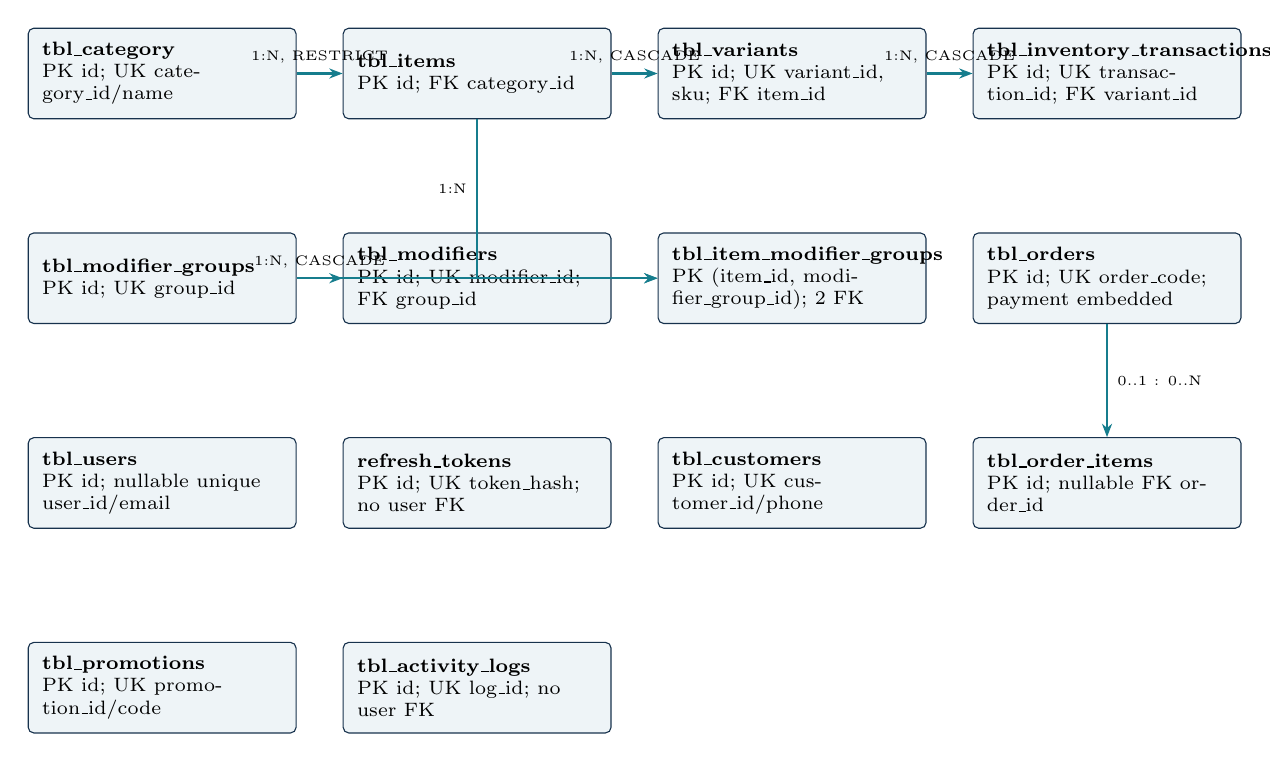
\begin{tikzpicture}[table/.style={draw=navy,rounded corners=2pt,fill=pale,align=left,text width=3.05cm,minimum height=1.15cm,font=\scriptsize,inner sep=5pt},edge/.style={-{Stealth[length=1.7mm]},draw=teal,thick}]
\node[table] (cat) at (0,5.5) {\textbf{tbl\_category}\\PK id; UK category\_id/name};
\node[table] (items) at (4,5.5) {\textbf{tbl\_items}\\PK id; FK category\_id};
\node[table] (vars) at (8,5.5) {\textbf{tbl\_variants}\\PK id; UK variant\_id, sku; FK item\_id};
\node[table] (inv) at (12,5.5) {\textbf{tbl\_inventory\_transactions}\\PK id; UK transaction\_id; FK variant\_id};
\node[table] (groups) at (0,2.9) {\textbf{tbl\_modifier\_groups}\\PK id; UK group\_id};
\node[table] (mods) at (4,2.9) {\textbf{tbl\_modifiers}\\PK id; UK modifier\_id; FK group\_id};
\node[table] (join) at (8,2.9) {\textbf{tbl\_item\_modifier\_groups}\\PK (item\_id, modifier\_group\_id); 2 FK};
\node[table] (orders) at (12,2.9) {\textbf{tbl\_orders}\\PK id; UK order\_code; payment embedded};
\node[table] (lines) at (12,0.3) {\textbf{tbl\_order\_items}\\PK id; nullable FK order\_id};
\node[table] (users) at (0,0.3) {\textbf{tbl\_users}\\PK id; nullable unique user\_id/email};
\node[table] (tokens) at (4,0.3) {\textbf{refresh\_tokens}\\PK id; UK token\_hash; no user FK};
\node[table] (customers) at (8,0.3) {\textbf{tbl\_customers}\\PK id; UK customer\_id/phone};
\node[table] (promos) at (0,-2.3) {\textbf{tbl\_promotions}\\PK id; UK promotion\_id/code};
\node[table] (logs) at (4,-2.3) {\textbf{tbl\_activity\_logs}\\PK id; UK log\_id; no user FK};
\draw[edge] (cat) -- node[above,font=\tiny]{1:N, RESTRICT} (items);
\draw[edge] (items) -- node[above,font=\tiny]{1:N, CASCADE} (vars);
\draw[edge] (vars) -- node[above,font=\tiny]{1:N, CASCADE} (inv);
\draw[edge] (groups) -- node[above,font=\tiny]{1:N, CASCADE} (mods);
\draw[edge] (items) |- node[pos=0.22,left,font=\tiny]{1:N} (join);
\draw[edge] (groups) -- (join);
\draw[edge] (orders) -- node[right,font=\tiny]{0..1 : 0..N} (lines);
\end{tikzpicture}
\caption{ERD vật lý: chỉ thể hiện các khóa ngoại khai báo trong migration V1}
\label{fig:erd-actual}
\end{figure}

\noindent\textbf{Mã Mermaid \texttt{erDiagram} — crow's foot cho schema thực tế:}
\begin{lstlisting}[style=mermaid,caption={ERD hiện thực theo 14 bảng trong migration V1},label={lst:erd-actual}]
erDiagram
  TBL_USERS {
    bigint id PK
    varchar user_id UK "nullable"
    varchar email UK "nullable"
    varchar role "nullable"
  }
  REFRESH_TOKENS {
    bigint id PK
    varchar token_hash UK
    varchar user_email
    varchar family_id
    timestamp expires_at
    timestamp revoked_at "nullable"
  }
  TBL_CATEGORY {
    bigint id PK
    varchar category_id UK "nullable"
    varchar name UK "nullable"
  }
  TBL_ITEMS {
    bigint id PK
    varchar item_id UK "nullable"
    bigint category_id FK
    decimal price "nullable"
  }
  TBL_VARIANTS {
    bigint id PK
    varchar variant_id UK
    varchar sku UK
    decimal base_price
    text attributes "nullable"
    int cached_stock_quantity
    bigint item_id FK
  }
  TBL_MODIFIER_GROUPS {
    bigint id PK
    varchar group_id UK
    int min_selections
    int max_selections
  }
  TBL_MODIFIERS {
    bigint id PK
    varchar modifier_id UK
    decimal price_adjustment
    bigint group_id FK
  }
  TBL_ITEM_MODIFIER_GROUPS {
    bigint item_id PK, FK
    bigint modifier_group_id PK, FK
  }
  TBL_CUSTOMERS {
    bigint id PK
    varchar customer_id UK
    varchar phone_number UK
    double total_spent
    int order_count
  }
  TBL_PROMOTIONS {
    bigint id PK
    varchar promotion_id UK
    varchar code UK "nullable"
    varchar days_of_week "nullable"
    int times_used
  }
  TBL_ORDERS {
    bigint id PK
    varchar order_code UK
    varchar customer_id "snapshot, no FK"
    varchar promotion_id "snapshot, no FK"
    tinyint status "ordinal"
    varchar payment_method
  }
  TBL_ORDER_ITEMS {
    bigint id PK
    bigint order_id FK "nullable"
    varchar item_id "no FK"
    varchar variant_id "no FK"
    text selected_modifiers "nullable"
  }
  TBL_INVENTORY_TRANSACTIONS {
    bigint id PK
    varchar transaction_id UK
    bigint variant_id FK
    varchar transaction_type
    int quantity
  }
  TBL_ACTIVITY_LOGS {
    bigint id PK
    varchar log_id UK
    varchar user_email
    varchar action
    varchar entity_id "polymorphic scalar"
  }
  TBL_CATEGORY ||--o{ TBL_ITEMS : contains
  TBL_ITEMS ||--o{ TBL_VARIANTS : defines
  TBL_ITEMS ||--o{ TBL_ITEM_MODIFIER_GROUPS : links
  TBL_MODIFIER_GROUPS ||--o{ TBL_ITEM_MODIFIER_GROUPS : links
  TBL_MODIFIER_GROUPS ||--o{ TBL_MODIFIERS : contains
  TBL_ORDERS o|--o{ TBL_ORDER_ITEMS : has_nullable_fk_lines
  TBL_VARIANTS ||--o{ TBL_INVENTORY_TRANSACTIONS : ledger
\end{lstlisting}

Mermaid marker \texttt{||--o\{} biểu diễn một parent với không hoặc nhiều dòng con; marker \texttt{o|--o\{} được dùng cho Order–OrderItem vì cột \texttt{order\_id} trong migration cho phép NULL. Liên kết Item–ModifierGroup là N:N ở mức khái niệm, nhưng trong ERD vật lý được triển khai qua \texttt{tbl\_item\_modifier\_groups}. Mermaid hỗ trợ các ký hiệu này trong ER diagram \cite{mermaider}. Sơ đồ có 1:N và N:N qua bảng nối; 1:1 hiện chưa được lưu bằng bảng riêng. Bảng \texttt{tbl\_users}, \texttt{refresh\_tokens}, \texttt{tbl\_customers}, \texttt{tbl\_promotions} và \texttt{tbl\_activity\_logs} không được nối tới nhau ở hình thực tế khi thiếu FK.

\section{Danh mục khóa, nullability và ràng buộc thực tế}
Tất cả bảng dùng khóa nội bộ \texttt{id BIGINT AUTO\_\allowbreak INCREMENT} làm PK, ngoại trừ bảng nối có PK ghép \texttt{(item\_\allowbreak id, modifier\_\allowbreak group\_\allowbreak id)}. Cột business ID có unique index nhằm nhận diện tài nguyên. Tuy nhiên, unique index trên cột cho phép NULL không đồng nghĩa với candidate key theo nghĩa quan hệ: MySQL cho phép nhiều NULL ở unique index; vì vậy các khóa business nullable trong migration được ghi là “unique index nullable”, không được gọi là candidate key tuyệt đối. Quy tắc CHECK và FK được diễn giải theo tài liệu MySQL \cite{mysqlfk,mysqlcheck}.

\small\begin{longtable}{@{}D{2.2cm}D{1.2cm}D{3.1cm}D{4.1cm}D{4.1cm}@{}}
\caption{Khóa, unique index, FK và nullability đáng chú ý của schema thực tế}\\
\toprule Bảng & PK & Candidate/unique key & FK và hành động xóa & NOT NULL ngoài PK\\\midrule
\endfirsthead
\toprule Bảng & PK & Candidate/unique key & FK và hành động xóa & NOT NULL ngoài PK\\\midrule
\endhead
\bottomrule\endfoot
tbl\_\allowbreak users & id & user\_\allowbreak id, email (unique nhưng nullable) & Không có & Không có trong migration\\
refresh\_\allowbreak tokens & id & token\_\allowbreak hash & Không có FK tới User & token\_\allowbreak hash, user\_\allowbreak email, family\_\allowbreak id, issued\_\allowbreak at, expires\_\allowbreak at\\
tbl\_\allowbreak category & id & category\_\allowbreak id, name (unique nhưng nullable) & Không có & Không có\\
tbl\_\allowbreak items & id & item\_\allowbreak id (unique nhưng nullable) & category\_\allowbreak id → category.id, RESTRICT & category\_\allowbreak id\\
tbl\_\allowbreak variants & id & variant\_\allowbreak id, sku & item\_\allowbreak id → items.id, CASCADE & variant\_\allowbreak id, sku, base\_\allowbreak price, cached\_\allowbreak stock\_\allowbreak quantity, item\_\allowbreak id\\
tbl\_\allowbreak modifier\_\allowbreak groups & id & group\_\allowbreak id & Không có & group\_\allowbreak id, name, min\_\allowbreak selections, max\_\allowbreak selections\\
tbl\_\allowbreak modifiers & id & modifier\_\allowbreak id & group\_\allowbreak id → modifier\_\allowbreak groups.id, CASCADE & modifier\_\allowbreak id, name, price\_\allowbreak adjustment, group\_\allowbreak id\\
tbl\_\allowbreak item\_\allowbreak modifier\_\allowbreak groups & cột ghép & (item\_\allowbreak id, modifier\_\allowbreak group\_\allowbreak id) & item/group → cha, CASCADE & item\_\allowbreak id, modifier\_\allowbreak group\_\allowbreak id\\
tbl\_\allowbreak customers & id & customer\_\allowbreak id, phone\_\allowbreak number & Không có & customer\_\allowbreak id, name, phone\_\allowbreak number, total\_\allowbreak spent, order\_\allowbreak count\\
tbl\_\allowbreak promotions & id & promotion\_\allowbreak id; code unique nullable & Không có & promotion\_\allowbreak id, name, type, discount\_\allowbreak value, min\_\allowbreak order\_\allowbreak amount, times\_\allowbreak used, is\_\allowbreak active\\
tbl\_\allowbreak orders & id & order\_\allowbreak code & Không có FK tới Customer/Promotion & order\_\allowbreak code\\
tbl\_\allowbreak order\_\allowbreak items & id & Không có unique business key & order\_\allowbreak id → orders.id, CASCADE; cột nullable & Không có\\
tbl\_\allowbreak inventory\_\allowbreak transactions & id & transaction\_\allowbreak id & variant\_\allowbreak id → variants.id, CASCADE & transaction\_\allowbreak id, variant\_\allowbreak id, transaction\_\allowbreak type, quantity\\
tbl\_\allowbreak activity\_\allowbreak logs & id & log\_\allowbreak id & Không có FK tới User & log\_\allowbreak id, user\_\allowbreak email, action, created\_\allowbreak at\\
\end{longtable}\normalsize

Migration không khai báo \texttt{CHECK}. Các ràng buộc NOT NULL của DB yếu hơn một số annotation JPA hoặc yêu cầu nghiệp vụ: ví dụ tbl\_users cho phép NULL ở email/password/role; tbl\_items cho phép NULL ở name/price; tbl\_order\_items chỉ bắt buộc id; tbl\_orders chỉ bắt buộc id/order\_code. Đây là mô tả DDL hiện tại, không phải khuyến nghị cho dữ liệu mới. Unique index trên promotions.code hoặc category.name nullable chỉ duy nhất với các giá trị khác NULL.

Các hành động ON DELETE được khai báo rõ trong V1 gồm: category→item RESTRICT; item→variant CASCADE; modifier group→modifier CASCADE; item/group→bảng nối CASCADE; order→order item CASCADE; variant→inventory transaction CASCADE. Không FK nào khai báo ON UPDATE; MySQL InnoDB áp dụng mặc định NO ACTION, tương đương RESTRICT tức chặn thay đổi khóa cha khi có dòng con tham chiếu \cite{mysqlfk}. Cascade xóa transaction lịch sử khi xóa Variant là lựa chọn đang có, dù có thể làm giảm khả năng giữ sổ cái lâu dài.

\section{Đánh giá chuẩn hóa lược đồ hiện tại}
Phân tích dưới đây xét lược đồ quan hệ theo dữ liệu lưu, không chỉ theo cách đặt tên entity. Khóa chính surrogate giúp định danh hàng; các thuộc tính mô tả chính không cho thấy phụ thuộc bộ phận trên khóa ghép ngoài bảng nối. Tuy nhiên, thiết kế vẫn có các vùng phi chuẩn hóa hoặc thiếu ràng buộc toàn vẹn cần ghi nhận:
\begin{enumerate}
\item \textbf{Giá trị nhiều phần/không nguyên tử:} \texttt{selected\_modifiers TEXT} gộp danh sách modifier của một dòng bán; \texttt{days\_of\_week} được service tách bằng dấu phẩy. Hai trường này biểu diễn tập phần tử trong một ô, nên không đạt 1NF dạng quan hệ chuẩn.
\item \textbf{Thuộc tính dẫn xuất lưu lặp:} \texttt{variants.cached\_stock\_quantity} được tính từ tổng ledger; \texttt{customers.total\_spent/order\_count} được cập nhật từ vòng đời đơn; \texttt{promotions.times\_used} là bộ đếm lượt sử dụng. Các giá trị này là projection/cache, cần đồng bộ với dữ liệu giao dịch gốc.
\item \textbf{Thiếu khóa ngoại:} order.customerId/promotionId, orderItem.itemId/variantId, refreshToken.userEmail và activityLog.userEmail là scalar không được FK bảo vệ. Dữ liệu mồ côi có thể được ghi nếu kiểm tra application thiếu hoặc có tác vụ DB ngoài ứng dụng.
\item \textbf{Snapshot giao dịch có chủ đích:} tên, giá, mã khách hàng/khuyến mãi tại thời điểm bán được sao chép vào order/order item. Các snapshot này có giá trị lịch sử và không nên bị nối ngược sang dữ liệu danh mục hiện tại để tính lại hóa đơn. Cần phân biệt snapshot nghiệp vụ với trùng lặp thiếu chủ ý.
\item \textbf{Ràng buộc miền chưa được DB thực thi:} Không có CHECK cho số lượng dòng, giá, trạng thái, discount, thứ tự ngày; nhiều cột nghiệp vụ nullable dù service mong đợi dữ liệu đầy đủ.
\end{enumerate}
Vì các điểm trên, kết luận phù hợp là: migration đang triển khai có các quan hệ và bảng nối đã chuẩn hóa một phần, nhưng không đủ căn cứ để khẳng định toàn bộ schema đạt 3NF nghiêm ngặt. Đặc biệt, 1NF chưa được bảo đảm với cột đa trị/serialized; do đó tuyên bố 3NF sẽ không chính xác theo định nghĩa quan hệ truyền thống.

\section{ERD 3NF đề xuất — tách khỏi hiện trạng}
Sơ đồ sau là phương án thiết kế học thuật; các bảng/khóa mới \textbf{chưa được triển khai trong V1}. Nó đưa mọi giá trị lặp/nhiều phần thành quan hệ riêng; thêm FK cho business associations; tách payment khỏi Order để biểu diễn 1:1; giữ snapshot giá/tên trong đơn như giá trị giao dịch bất biến. Stock/CRM/promotion counters được xem là view hoặc projection, không phải cột chuẩn hóa của bảng gốc.

\begin{figure}[htbp]
\centering
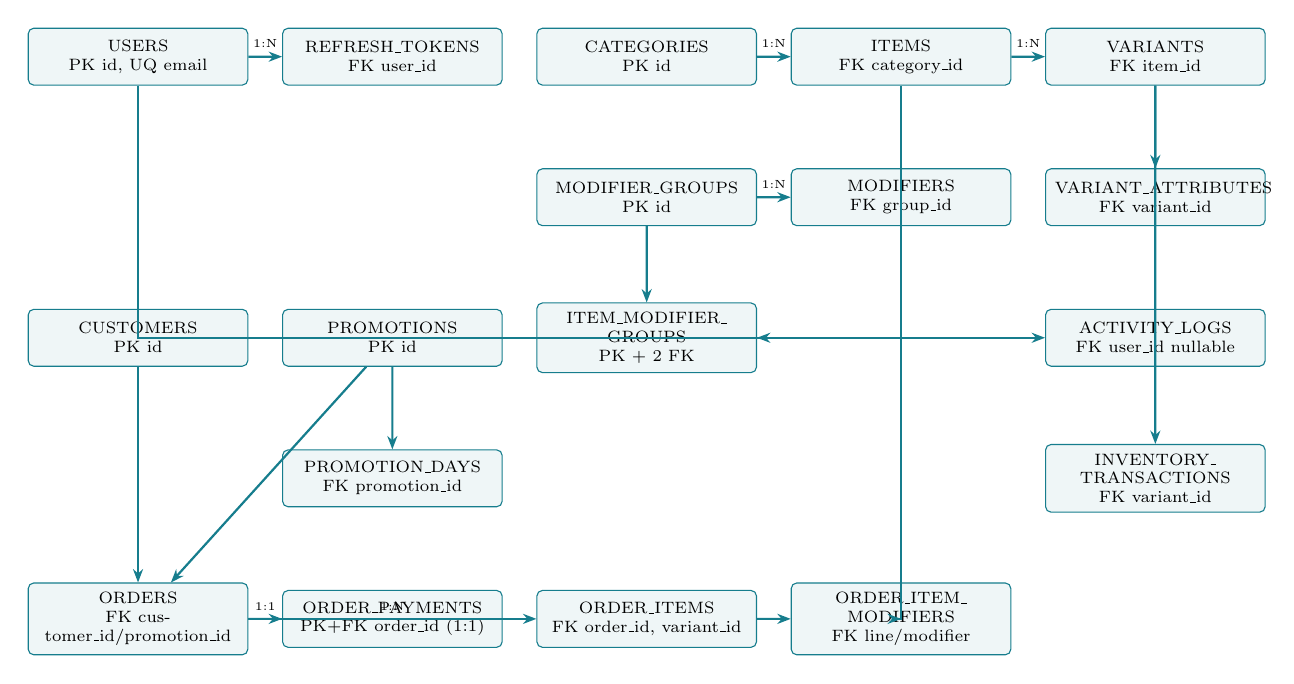
\begin{tikzpicture}[scale=0.85,transform shape,table/.style={draw=teal,rounded corners=2pt,fill=teal!7,align=center,text width=3.0cm,minimum height=0.85cm,font=\scriptsize,inner sep=4pt},edge/.style={-{Stealth[length=1.7mm]},draw=teal,thick}]
\node[table] (user2) at (0,5.3) {USERS\\PK id, UQ email};
\node[table] (token2) at (3.8,5.3) {REFRESH\_TOKENS\\FK user\_id};
\node[table] (cat2) at (7.6,5.3) {CATEGORIES\\PK id};
\node[table] (item2) at (11.4,5.3) {ITEMS\\FK category\_id};
\node[table] (variant2) at (15.2,5.3) {VARIANTS\\FK item\_id};
\node[table] (attrs2) at (15.2,3.2) {VARIANT\_ATTRIBUTES\\FK variant\_id};
\node[table] (group2) at (7.6,3.2) {MODIFIER\_GROUPS\\PK id};
\node[table] (mod2) at (11.4,3.2) {MODIFIERS\\FK group\_id};
\node[table] (link2) at (7.6,1.1) {ITEM\_\allowbreak MODIFIER\_\allowbreak GROUPS\\PK + 2 FK};
\node[table] (customer2) at (0,1.1) {CUSTOMERS\\PK id};
\node[table] (promo2) at (3.8,1.1) {PROMOTIONS\\PK id};
\node[table] (days2) at (3.8,-1.0) {PROMOTION\_DAYS\\FK promotion\_id};
\node[table] (order2) at (0,-3.1) {ORDERS\\FK customer\_id/promotion\_id};
\node[table] (payment2) at (3.8,-3.1) {ORDER\_PAYMENTS\\PK+FK order\_id (1:1)};
\node[table] (line2) at (7.6,-3.1) {ORDER\_ITEMS\\FK order\_id, variant\_id};
\node[table] (lineMod2) at (11.4,-3.1) {ORDER\_\allowbreak ITEM\_\allowbreak MODIFIERS\\FK line/modifier};
\node[table] (inv2) at (15.2,-1.0) {INVENTORY\_\allowbreak TRANSACTIONS\\FK variant\_id};
\node[table] (logs2) at (15.2,1.1) {ACTIVITY\_LOGS\\FK user\_id nullable};
\draw[edge] (user2) -- node[above,font=\tiny]{1:N} (token2);
\draw[edge] (cat2) -- node[above,font=\tiny]{1:N} (item2);
\draw[edge] (item2) -- node[above,font=\tiny]{1:N} (variant2);
\draw[edge] (variant2) -- (attrs2);
\draw[edge] (group2) -- node[above,font=\tiny]{1:N} (mod2);
\draw[edge] (item2) |- (link2);
\draw[edge] (group2) -- (link2);
\draw[edge] (customer2) -- (order2);
\draw[edge] (promo2) -- (order2);
\draw[edge] (promo2) -- (days2);
\draw[edge] (order2) -- node[above,font=\tiny]{1:1} (payment2);
\draw[edge] (order2) -- node[above,font=\tiny]{1:N} (line2);
\draw[edge] (line2) -- (lineMod2);
\draw[edge] (mod2) |- (lineMod2);
\draw[edge] (variant2) -- (inv2);
\draw[edge] (user2) |- (logs2);
\end{tikzpicture}
\caption{ERD 3NF đề xuất — thiết kế mục tiêu, chưa triển khai}
\label{fig:erd-target}
\end{figure}

\noindent\textbf{Mã Mermaid đề xuất, gồm 1:1, 1:N và N:N qua bảng nối:}
\begin{lstlisting}[style=mermaid,caption={ERD mục tiêu chuẩn hóa — không đồng nhất với migration hiện hành},label={lst:erd-3nf}]
erDiagram
  USERS ||--o{ REFRESH_TOKENS : owns
  USERS o|--o{ ACTIVITY_LOGS : performs
  CATEGORIES ||--o{ ITEMS : classifies
  ITEMS ||--o{ VARIANTS : defines
  VARIANTS ||--o{ VARIANT_ATTRIBUTES : has_atomic_attributes
  ITEMS ||--o{ ITEM_MODIFIER_GROUPS : links
  MODIFIER_GROUPS ||--o{ ITEM_MODIFIER_GROUPS : links
  MODIFIER_GROUPS ||--o{ MODIFIERS : contains
  PROMOTIONS ||--o{ PROMOTION_DAYS : applies_on
  CUSTOMERS o|--o{ ORDERS : associated_customer
  PROMOTIONS o|--o{ ORDERS : applied_promotion
  ORDERS ||--|| ORDER_PAYMENTS : payment_details
  ORDERS ||--o{ ORDER_ITEMS : contains
  VARIANTS ||--o{ ORDER_ITEMS : sold_variant
  ORDER_ITEMS ||--o{ ORDER_ITEM_MODIFIERS : snapshots
  MODIFIERS ||--o{ ORDER_ITEM_MODIFIERS : selected_modifier
  VARIANTS ||--o{ INVENTORY_TRANSACTIONS : ledger

  USERS {
    bigint id PK
    varchar email UK
  }
  REFRESH_TOKENS {
    bigint id PK
    bigint user_id FK
    varchar token_hash UK
    varchar family_id
  }
  CATEGORIES {
    bigint id PK
    varchar category_id UK
  }
  ITEMS {
    bigint id PK
    bigint category_id FK
    varchar item_id UK
  }
  VARIANTS {
    bigint id PK
    bigint item_id FK
    varchar sku UK
    decimal base_price
  }
  VARIANT_ATTRIBUTES {
    bigint variant_id PK, FK
    varchar attribute_name PK
    varchar attribute_value
  }
  MODIFIER_GROUPS {
    bigint id PK
    varchar group_id UK
  }
  MODIFIERS {
    bigint id PK
    bigint group_id FK
    varchar modifier_id UK
  }
  ITEM_MODIFIER_GROUPS {
    bigint item_id PK, FK
    bigint modifier_group_id PK, FK
  }
  CUSTOMERS {
    bigint id PK
    varchar customer_id UK
    varchar phone_number UK
  }
  PROMOTIONS {
    bigint id PK
    varchar promotion_id UK
    varchar code UK
  }
  PROMOTION_DAYS {
    bigint promotion_id PK, FK
    tinyint day_of_week PK
  }
  ORDERS {
    bigint id PK
    bigint customer_id FK "nullable"
    bigint promotion_id FK "nullable"
    varchar order_code UK
  }
  ORDER_PAYMENTS {
    bigint order_id PK, FK
    varchar method
    varchar status
    varchar payment_link_id
  }
  ORDER_ITEMS {
    bigint id PK
    bigint order_id FK
    bigint variant_id FK
    int quantity
    decimal unit_price_snapshot
  }
  ORDER_ITEM_MODIFIERS {
    bigint id PK
    bigint order_item_id FK
    bigint modifier_id FK
    decimal price_snapshot
  }
  INVENTORY_TRANSACTIONS {
    bigint id PK
    bigint variant_id FK
    varchar transaction_type
    int signed_quantity
  }
  ACTIVITY_LOGS {
    bigint id PK
    bigint user_id FK "nullable"
    varchar user_email_snapshot
  }
\end{lstlisting}

Trong phương án này, Item–ModifierGroup vẫn là N:N nhưng được phân rã bởi bảng nối có khóa chính ghép. Order–OrderPayment là 1:1 thông qua việc cột \texttt{order\_id} đồng thời là PK và FK. Order–OrderItem là 1:N; Order–Customer/Promotion là tùy chọn ở phía Order. Variant–Attribute và Promotion–Day tách các tập giá trị khỏi ô text. OrderItem–Modifier được phân rã bằng bảng nối có cột snapshot giá để không phụ thuộc giá Modifier đang có tại thời điểm đọc lịch sử.

\subsection{Ràng buộc toàn vẹn nên khai báo trong thiết kế mục tiêu}
Các quy tắc sau là đề xuất cho migration tương lai. Chúng không xuất hiện như CHECK trong V1, do đó không được gắn nhãn đã cưỡng chế ở database.
\small\begin{longtable}{@{}D{2.3cm}D{3.1cm}D{6.1cm}D{3.4cm}@{}}
\caption{Danh mục NOT NULL/UNIQUE/CHECK đề xuất}\\
\toprule Phân hệ & Ràng buộc đề xuất & Quy tắc & Trạng thái hiện tại\\\midrule
\endfirsthead
\toprule Phân hệ & Ràng buộc đề xuất & Quy tắc & Trạng thái hiện tại\\\midrule
\endhead
\bottomrule\endfoot
Tài khoản & NOT NULL + UNIQUE & email, password hash, role; email là candidate key khi NOT NULL. user\_\allowbreak id có thể là alternate key nếu bắt buộc nhập. & Email/user\_\allowbreak id nullable trong V1.\\
Refresh token & NOT NULL + UNIQUE & token\_\allowbreak hash duy nhất; user\_\allowbreak id FK; expires\_\allowbreak at lớn hơn issued\_\allowbreak at; family\_\allowbreak id NOT NULL. & Hash/family/time bắt buộc; chưa có FK user.\\
Danh mục & NOT NULL + UNIQUE & category\_\allowbreak id/name bắt buộc nếu mỗi danh mục phải định danh duy nhất; unique key trên name theo quy tắc cửa hàng. & Các cột nullable.\\
Biến thể & CHECK + FK & base\_\allowbreak price $>$ 0; cached stock không ràng buộc không âm vì cho phép tồn âm; item\_\allowbreak id bắt buộc. & NOT NULL/FK một phần; chưa CHECK.\\
ModifierGroup & CHECK & min\_\allowbreak selections $\geq 0$; max\_\allowbreak selections $\geq$ min\_\allowbreak selections. & NOT NULL; không CHECK.\\
Order item & NOT NULL + CHECK + FK & order\_\allowbreak id/variant\_\allowbreak id/quantity bắt buộc; quantity $>$ 0; unit\_\allowbreak price\_\allowbreak snapshot $\geq 0$. & order\_\allowbreak id/quantity/IDs nullable; không CHECK.\\
Payment & NOT NULL + CHECK & order\_\allowbreak id unique/PK; method thuộc CASH/PAYOS; status thuộc một trong bốn giá trị PENDING, COMPLETED, FAILED, CANCELLED. & Embedded; status ordinal TINYINT; không CHECK.\\
Khuyến mãi & CHECK & discount value/min order/max discount không âm; ngày bắt đầu không sau ngày kết thúc; discount percent $\leq 100$; BOGO percent thuộc [0,100]. & Không CHECK.\\
Kho & CHECK theo loại & IN có signed quantity $>$ 0; OUT $<$ 0; ADJUSTMENT có thể âm/bằng 0/dương. & Không CHECK; service ký dấu ở application.\\
CRM & Dẫn xuất & total\_\allowbreak spent/order\_\allowbreak count nên là view/projection; nếu giữ cache thì giá trị không âm và cập nhật giao dịch nguyên tử. & Cột lưu trực tiếp; không CHECK.\\
Promotion days/attributes & PK ghép + FK & (promotion\_\allowbreak id, day); (variant\_\allowbreak id, attribute\_\allowbreak name) duy nhất để tách tập giá trị. & Cả hai dùng scalar/string hiện tại.\\
\end{longtable}\normalsize

\subsection{ON DELETE/ON UPDATE cho quan hệ đề xuất}
Khóa chính surrogate được xem là bất biến; mọi FK mục tiêu nên khai báo \texttt{ON UPDATE RESTRICT/NO ACTION}. Với InnoDB, khi bỏ qua ON UPDATE, NO ACTION/RESTRICT được dùng mặc định \cite{mysqlfk}. Khuyến nghị delete policy giữ bản ghi có giá trị kiểm toán, đồng thời giao dịch xóa chỉ qua service được ủy quyền:
\begin{table}[htbp]
\centering\small
\caption{Chính sách tham chiếu đề xuất}
\begin{tabularx}{\textwidth}{@{}p{3.5cm}p{4.2cm}p{3.1cm}Y@{}}\toprule
Quan hệ FK & ON DELETE đề xuất & ON UPDATE & Lý do\\\midrule
Category → Item & RESTRICT & RESTRICT & Không bỏ danh mục đang phân loại sản phẩm.\\
Item → Variant & RESTRICT hoặc soft delete & RESTRICT & Không xóa SKU đang được dùng bởi lịch sử bán/kho.\\
Item/ModifierGroup → bảng nối & CASCADE & RESTRICT & Xóa liên kết thuần cấu hình; không làm mất dòng giao dịch đã snapshot.\\
ModifierGroup → Modifier & RESTRICT/soft delete & RESTRICT & Modifier cũ có thể được tham chiếu từ OrderItemModifier.\\
Customer/Promotion → Order & SET NULL & RESTRICT & Giữ hóa đơn và snapshot nếu hồ sơ chủ bị xóa; FK tùy chọn.\\
Order → OrderPayment & CASCADE & RESTRICT & Quan hệ 1:1 phụ thuộc vòng đời đơn; xóa đơn được kiểm soát ở service.\\
Order → OrderItem → OrderItemModifier & CASCADE & RESTRICT & Dọn cấu trúc con khi xóa đơn đủ điều kiện; không áp dụng cho đơn COMPLETED.\\
Variant → InventoryTransaction & RESTRICT & RESTRICT & Không xóa ledger lịch sử khi SKU bị xóa; ưu tiên archive/soft delete.\\
User → RefreshToken & CASCADE & RESTRICT & Xóa tài khoản phải thu hồi các phiên liên quan.\\
User → ActivityLog & SET NULL & RESTRICT & Giữ audit record; lưu email snapshot để còn dấu vết.\\
\bottomrule\end{tabularx}
\end{table}

\section{Ma trận khoảng cách giữa schema hiện tại và thiết kế 3NF}
\begin{table}[htbp]
\centering\small
\caption{Các thay đổi dữ liệu cần có nếu chuyển từ V1 sang mô hình 3NF đề xuất}
\begin{tabularx}{\textwidth}{@{}p{4.2cm}p{4.3cm}Y@{}}\toprule
Hiện trạng V1 & Thiết kế mục tiêu & Ảnh hưởng tới ứng dụng\\\midrule
selected\_modifiers là TEXT trên tbl\_order\_items & Tạo ORDER\_\allowbreak ITEM\_\allowbreak MODIFIERS, lưu mỗi lựa chọn thành một dòng cùng snapshot tên/giá & Cập nhật mapper/DTO và truy vấn chi tiết đơn; giữ khả năng tái hiện giá cũ.\\
days\_of\_week là chuỗi phân tách dấu phẩy & Tạo PROMOTION\_DAYS một dòng cho mỗi thứ áp dụng & Thay logic split chuỗi bằng query/collection quan hệ.\\
attributes là JSON map trong TEXT & Tạo VARIANT\_ATTRIBUTES với khóa ghép variant/name & Làm tăng số dòng nhưng tạo truy vấn ràng buộc kiểu thuộc tính rõ ràng.\\
Order.customerId / promotionId scalar & Thêm FK customer\_id/promotion\_id và giữ snapshot lịch sử & Chính sách xóa phải dùng SET NULL/soft delete để không mất hóa đơn.\\
OrderItem.itemId/variantId scalar & OrderItem gắn FK đến Variant; tên/giá bán giữ dạng snapshot & Thống nhất Variant là đơn vị bán/tồn; cần migration dữ liệu legacy.\\
PaymentDetails nhúng trong Order & Tách ORDER\_PAYMENTS với order\_id vừa PK vừa FK & Tạo quan hệ bảng 1:1, dễ mở rộng attempt/transaction sau này.\\
stock/CRM/promotion counters lưu trực tiếp & Tính bằng view hoặc read projection rõ ràng & Cần cân đối hiệu năng với độ nhất quán; nếu giữ cache phải có rebuild/monitor.\\
\bottomrule\end{tabularx}
\end{table}

\chapter*{KẾT LUẬN VÀ GIỚI HẠN ĐẶC TẢ}
\addcontentsline{toc}{chapter}{KẾT LUẬN VÀ GIỚI HẠN ĐẶC TẢ}
Báo cáo đã mô tả actor, biên hệ thống, các use case chính, mô hình miền, lớp nghiệp vụ trọng tâm và quan hệ dữ liệu theo code Billing-app khảo sát. Đặc điểm thiết kế nổi bật là quy trình xử lý đơn QR xuyên qua PayOS; ledger có signed quantity là nguồn tính tồn; cancellation là một thao tác bù trừ nhiều phân hệ; refresh token được xoay vòng theo family; và một số thông tin khách hàng/khuyến mãi được chụp thành snapshot trong đơn.

Kết quả phân tích cũng cho thấy cần phân biệt invariant ứng dụng với ràng buộc DB. Việc chặn xóa đơn COMPLETED nằm ở service, không nằm trong CHECK/trigger; nhiều trường trong bảng có thể NULL; một số mã tham chiếu không có FK; migration không có CHECK; cột modifier/ngày áp dụng chứa cấu trúc nhiều phần; và một số trường tồn/CRM/promotion là cache. Do đó ERD triển khai không được mô tả là 3NF nghiêm ngặt. ERD 3NF riêng đưa ra hướng tách giá trị đa trị, khóa ngoại và payment 1:1, song đây là thiết kế mục tiêu chứ chưa phải trạng thái đã cài đặt.

Những nội dung chưa được xác nhận gồm: chỉ tiêu hiệu năng/availability, khả năng offline đồng bộ đầy đủ, chính sách lưu trữ lịch sử lâu dài, mức idempotency của webhook, chiến lược xử lý payment callback trễ và bảo đảm commit việc thu hồi token family khi replay. Báo cáo không gán kết quả kiểm thử pass/fail; đây là đặc tả được suy ra từ cấu hình và source đã khảo sát, không phải biên bản kiểm thử nghiệm thu.

\begin{thebibliography}{99}
\bibitem{iso29148} ISO/IEC/IEEE, \textit{ISO/IEC/IEEE 29148:2018 — Systems and software engineering: Life cycle processes — Requirements engineering}, 2nd ed., 2018. Bản này được ISO rà soát/duy trì hiệu lực năm 2024. [Trực tuyến] \url{https://www.iso.org/standard/72089.html}.
\bibitem{uml} Object Management Group, \textit{OMG Unified Modeling Language (OMG UML), Version 2.5.1}, Dec. 2017. [Trực tuyến] \url{https://www.omg.org/spec/UML/2.5.1/About-UML}.
\bibitem{mermaidclass} Mermaid, \textit{Class diagrams syntax}. [Trực tuyến] \url{https://mermaid.js.org/syntax/classDiagram.html}.
\bibitem{mermaider} Mermaid, \textit{Entity Relationship Diagrams syntax}. [Trực tuyến] \url{https://mermaid.js.org/syntax/entityRelationshipDiagram.html}.
\bibitem{mysqlfk} Oracle, \textit{MySQL 8.4 Reference Manual, Foreign Key Constraints}. [Trực tuyến] \url{https://dev.mysql.com/doc/refman/8.4/en/create-table-foreign-keys.html}.
\bibitem{mysqlcheck} Oracle, \textit{MySQL 8.4 Reference Manual, CHECK Constraints}. [Trực tuyến] \url{https://dev.mysql.com/doc/refman/8.4/en/create-table-check-constraints.html}.
\bibitem{springtx} Spring Framework, \textit{@Transactional API and rollback defaults}. [Trực tuyến] \url{https://docs.spring.io/spring-framework/docs/current/javadoc-api/org/springframework/transaction/annotation/Transactional.html}.
\bibitem{context} Billing-app, \textit{CONTEXT.md}, tài liệu tổng quan hệ thống trong repository, khảo sát ngày 24/09/2026.
\bibitem{schema} Billing-app, \textit{billingsoftware/src/main/resources/db/migration/V1\_\_init\_schema.sql}, migration Flyway, khảo sát ngày 24/09/2026.
\bibitem{adr} Billing-app, \textit{docs/adr/0001--0009}, quyết định kiến trúc, đối chiếu với mã triển khai ngày 24/09/2026.
\bibitem{ordercode} Billing-app, \textit{OrderController.java; OrderServiceImpl.java; OrderEntity.java; OrderItemEntity.java; PaymentWebhookController.java}, mã nguồn backend.
\bibitem{inventorycode} Billing-app, \textit{InventoryController.java; InventoryServiceImpl.java; InventoryTransactionEntity.java; VariantEntity.java}, mã nguồn backend.
\bibitem{authcode} Billing-app, \textit{AuthController.java; RefreshTokenService.java; RefreshTokenEntity.java; SecurityConfig.java}, mã nguồn backend.
\bibitem{promotioncode} Billing-app, \textit{PromotionServiceImpl.java; PromotionEntity.java; CustomerEntity.java; ActivityLogServiceImpl.java}, mã nguồn backend.
\end{thebibliography}

\end{document}
